\chapter{ОБЗОР МОДЕЛЕЙ ТРЕЩИНЫ ГИДРОРАЗРЫВА ПЛАСТА} \label{ch1}

В настоящее время в симуляторах для моделирования процесса гидроразрыва пласта (ГРП) нефтяные компании используют модели Pseudo3D, Planar3D и Full3D.

Наиболее общая модель Full3D позволяет моделировать сложные варианты развития трещины (учитывается возможность изменения направления распространения трещины и слоистость породы), решение проводится численно с применением метода конечных элементов (МКЭ), но эта модель используется редко, так как имеет низкую скорость расчёта.
Основным преимуществом модели Full3D по сравнению со всеми другими моделями является отсутствие допущений относительно геометрии трещины, что позволяет моделировать изменение направления распространения трещин (например, за счёт их взаимовлияния).

В модели Planar3D предполагается, что направление минимальных горизонтальных напряжений в пласте не изменяется, то есть трещина распространяется в одной плоскости, перпендикулярной минимальным горизонтальным напряжениям в породе.
В то же время модель Planar3D учитывает слоистость породы и не использует приближение малости высоты в сравнении с длиной трещины, то есть учитывает двумерное течение жидкости.

Модель Pseudo3D использует предположение о том, что высота трещины много меньше её длины и в каждом вертикальном сечении давление одинаково по сечению, то есть рассматривается случай одномерного течения жидкости.
Модели Pseudo3D при небольших вычислительных затратах дают хорошее представление о возможном развитии трещины ГРП и в зависимости от численной реализации разделяются на подвиды: Lumped-Pseudo3D, Cell-based-Pseudo3D \cite{adachi} и Semi-analytical-Pseudo3D \cite{shel_paderin}.

Каждая из моделей Pseudo3D, Planar3D и Full3D плохо поддаётся аналитическому анализу.
Однако при введении дополнительных предположений и допущений модель Planar3D преобразуется в хорошо известные модели (исторически были изучены раньше модели Planar3D), для которых можно провести аналитический анализ (найти длину, раскрытие и давление в трещине в зависимости от координаты и времени).
В \taref{tab:fracking_models} представлены основные модели трещины ГРП с их допущениями (использованы схематичные рисунки, заимствованные из работ \cite{adachi, dontsov_peirce, valov_baykin_dontsov, baykin_course}).

\newcolumntype{L}[1]{>{\raggedright\arraybackslash}m{#1}}
\noindent % for correct centering
\begingroup
\small %выставляем шрифт в 12bp
\begin{longtable}[l]{|L{2.2cm}|m{7.3cm}|L{6.2cm}|}
	\caption{Допущения основных моделей трещины ГРП}%
	\label{tab:fracking_models}% label всегда желательно идти после caption
	\\
	\hline
	\multicolumn{1}{|c|}{\textbf{Модель}}&\multicolumn{1}{|c|}{\textbf{Допущения}}&\multicolumn{1}{|c|}{\textbf{Схематичный рисунок}\footnotemark}\\ \hline
	\endfirsthead%
	\captionsetup{format=tablenocaption,labelformat=continued} % до caption!
	\caption[]{}\\ % печать слов о продолжении таблицы
	\hline
	\multicolumn{1}{|c|}{\textbf{Модель}}&\multicolumn{1}{|c|}{\textbf{Допущения}}&\multicolumn{1}{|c|}{\textbf{Схематичный рисунок}}\\ \hline
	\endhead
	\hline
	\endfoot
	\hline
	\endlastfoot
	Full3D\footnotetext{Схематичные рисунки заимствованы из работ Алексея Николаевича Байкина, Александра Викторовича Валова, Егора Владимировича Донцова \cite{dontsov_peirce, valov_baykin_dontsov, baykin_course} и J.Adachi et al. \cite{adachi}}&Отсутствуют; учёт большого количества физических эффектов позволяет очень точно (часто излишне точно) описать распространение трещины\break\hfill\break (рисунок заимствован из \cite{baykin_course}) &\hfill\break\makecell[c]{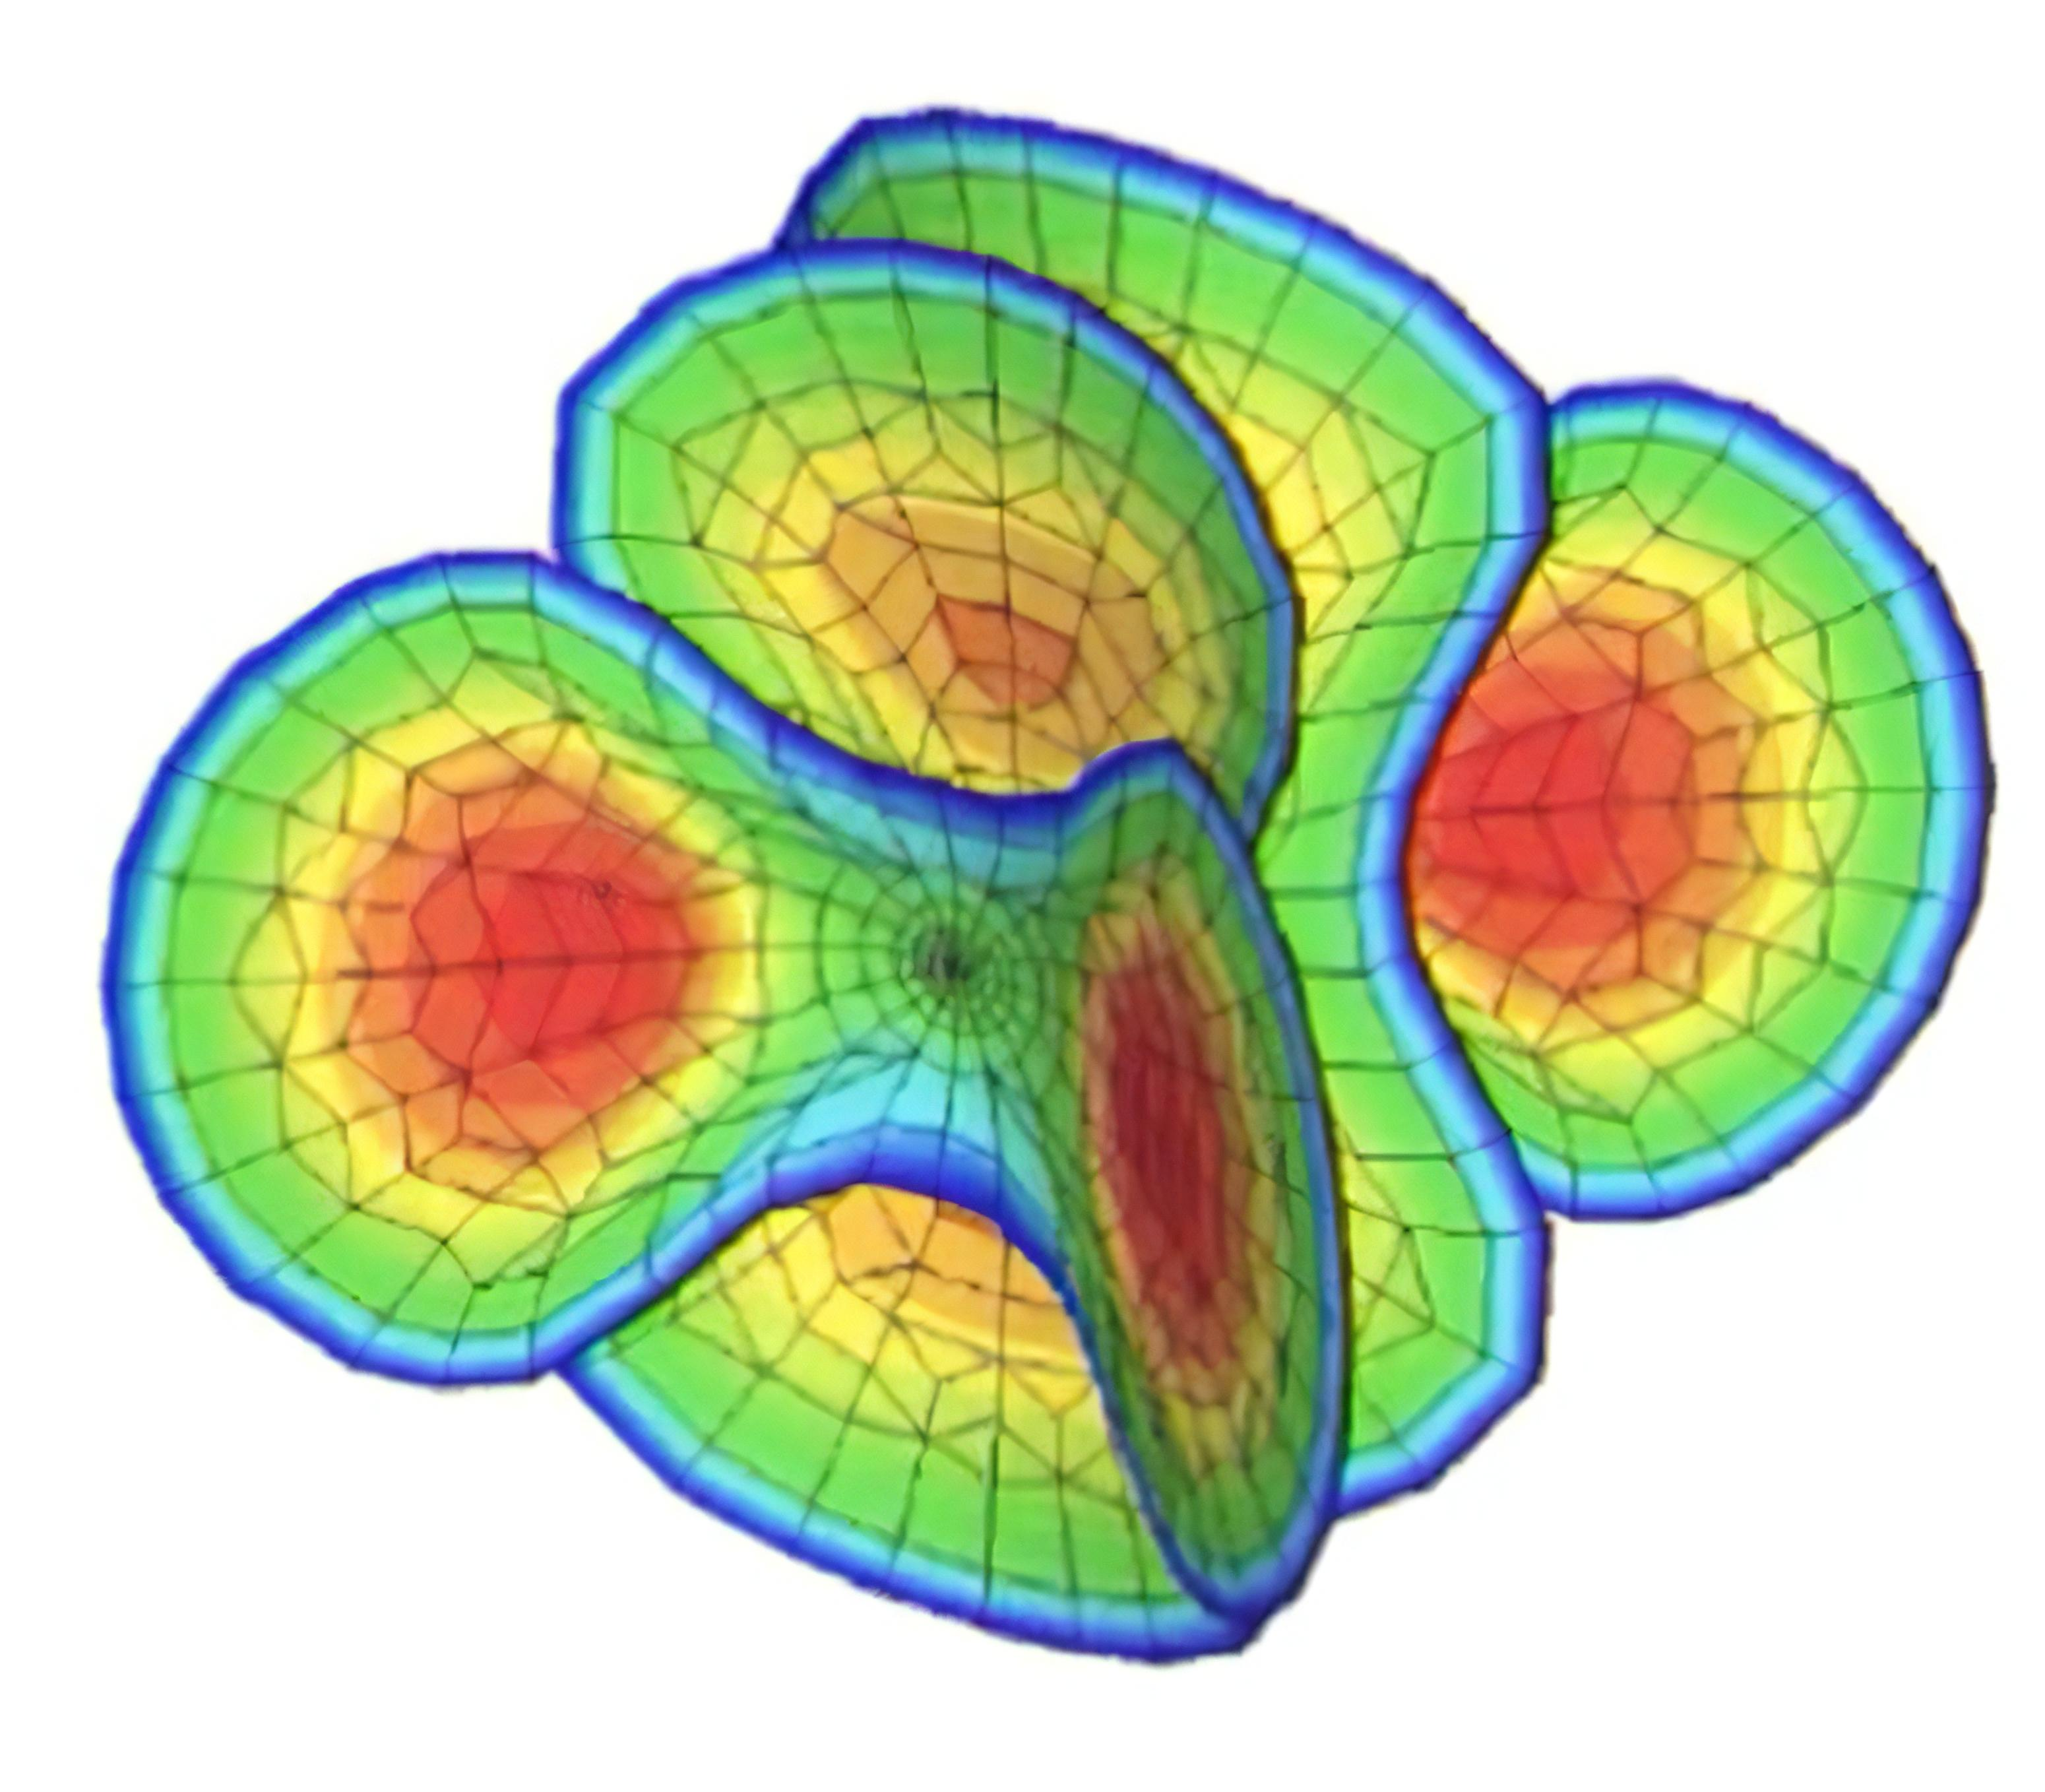
\includegraphics[width=0.6\linewidth]{images/full3D_scheme_better.jpg}}\hfill\break\\ \hline
	Planar3D&Одна планарная трещина, распространяющаяся в плоскости вдоль направления максимальных горизонтальных напряжений; законы упругости рассматриваются в рамках линейно-упругой механики разрушения в общем случае без дополнительных упрощений; поток жидкости вдоль трещины двумерный\break\hfill\break (рисунок заимствован из \cite{valov_baykin_dontsov})&\hfill\break\makecell[c]{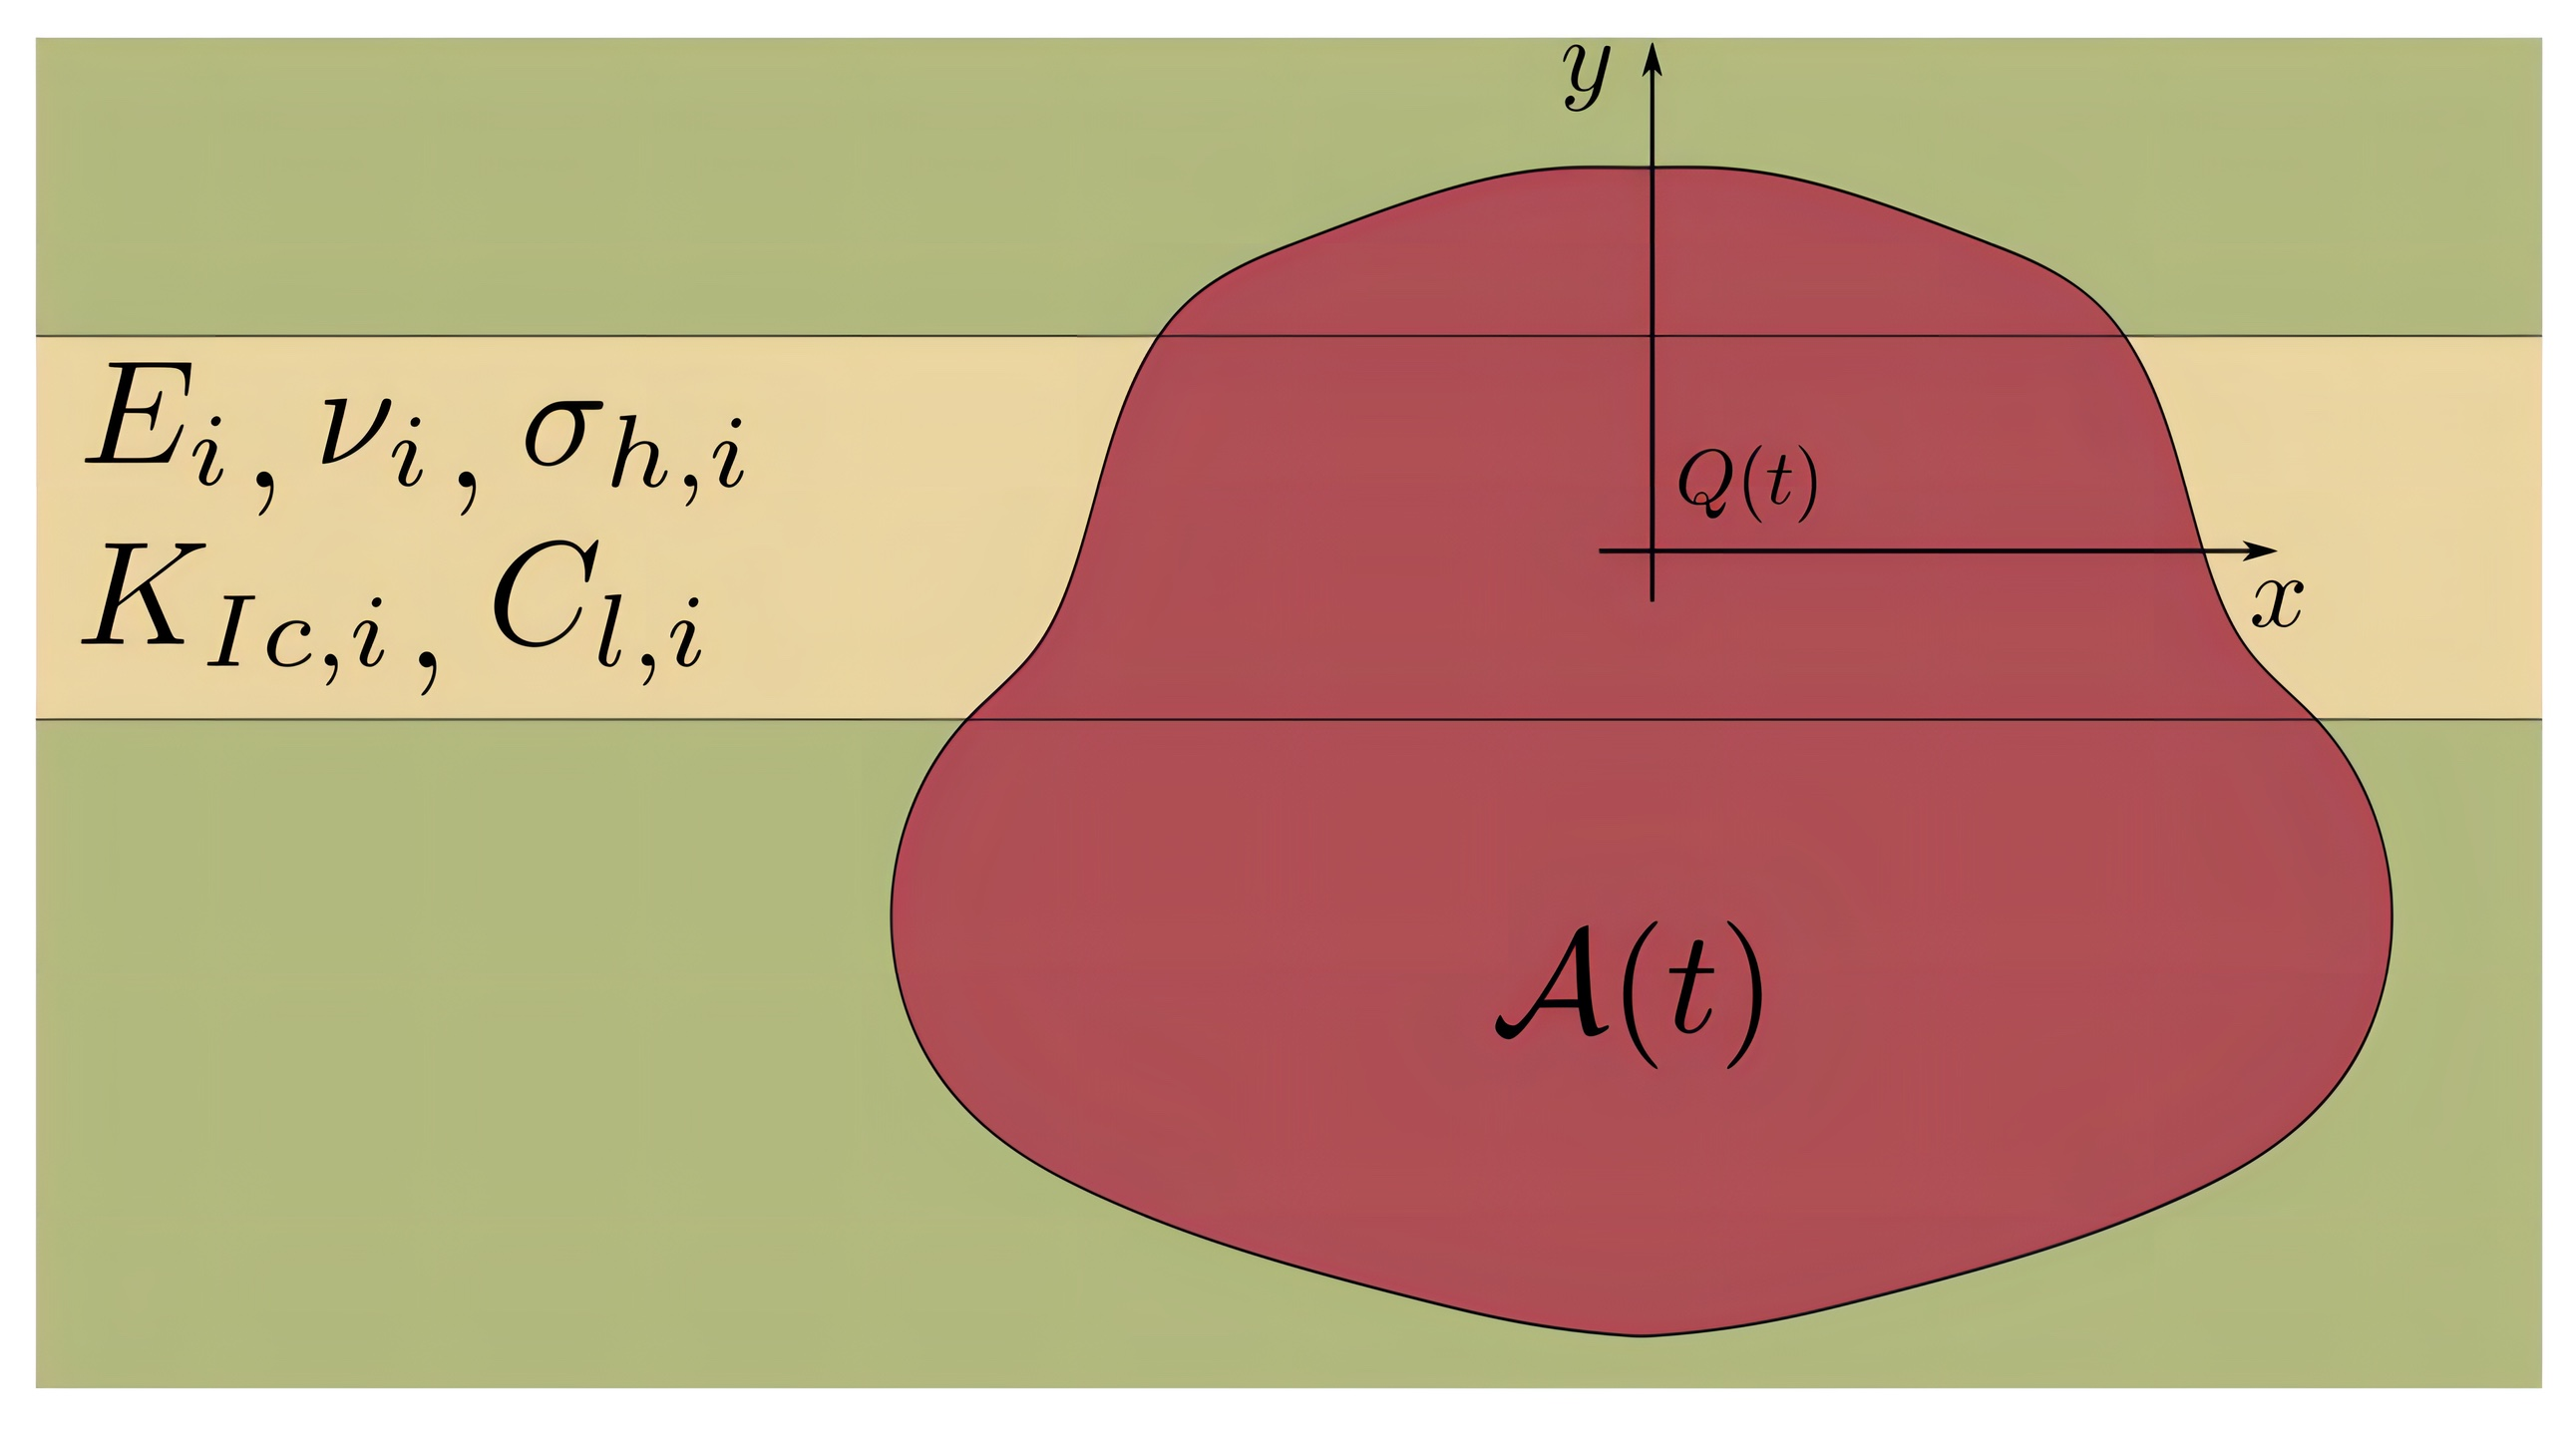
\includegraphics[width=\linewidth]{images/planar3D_model_new.jpg}\\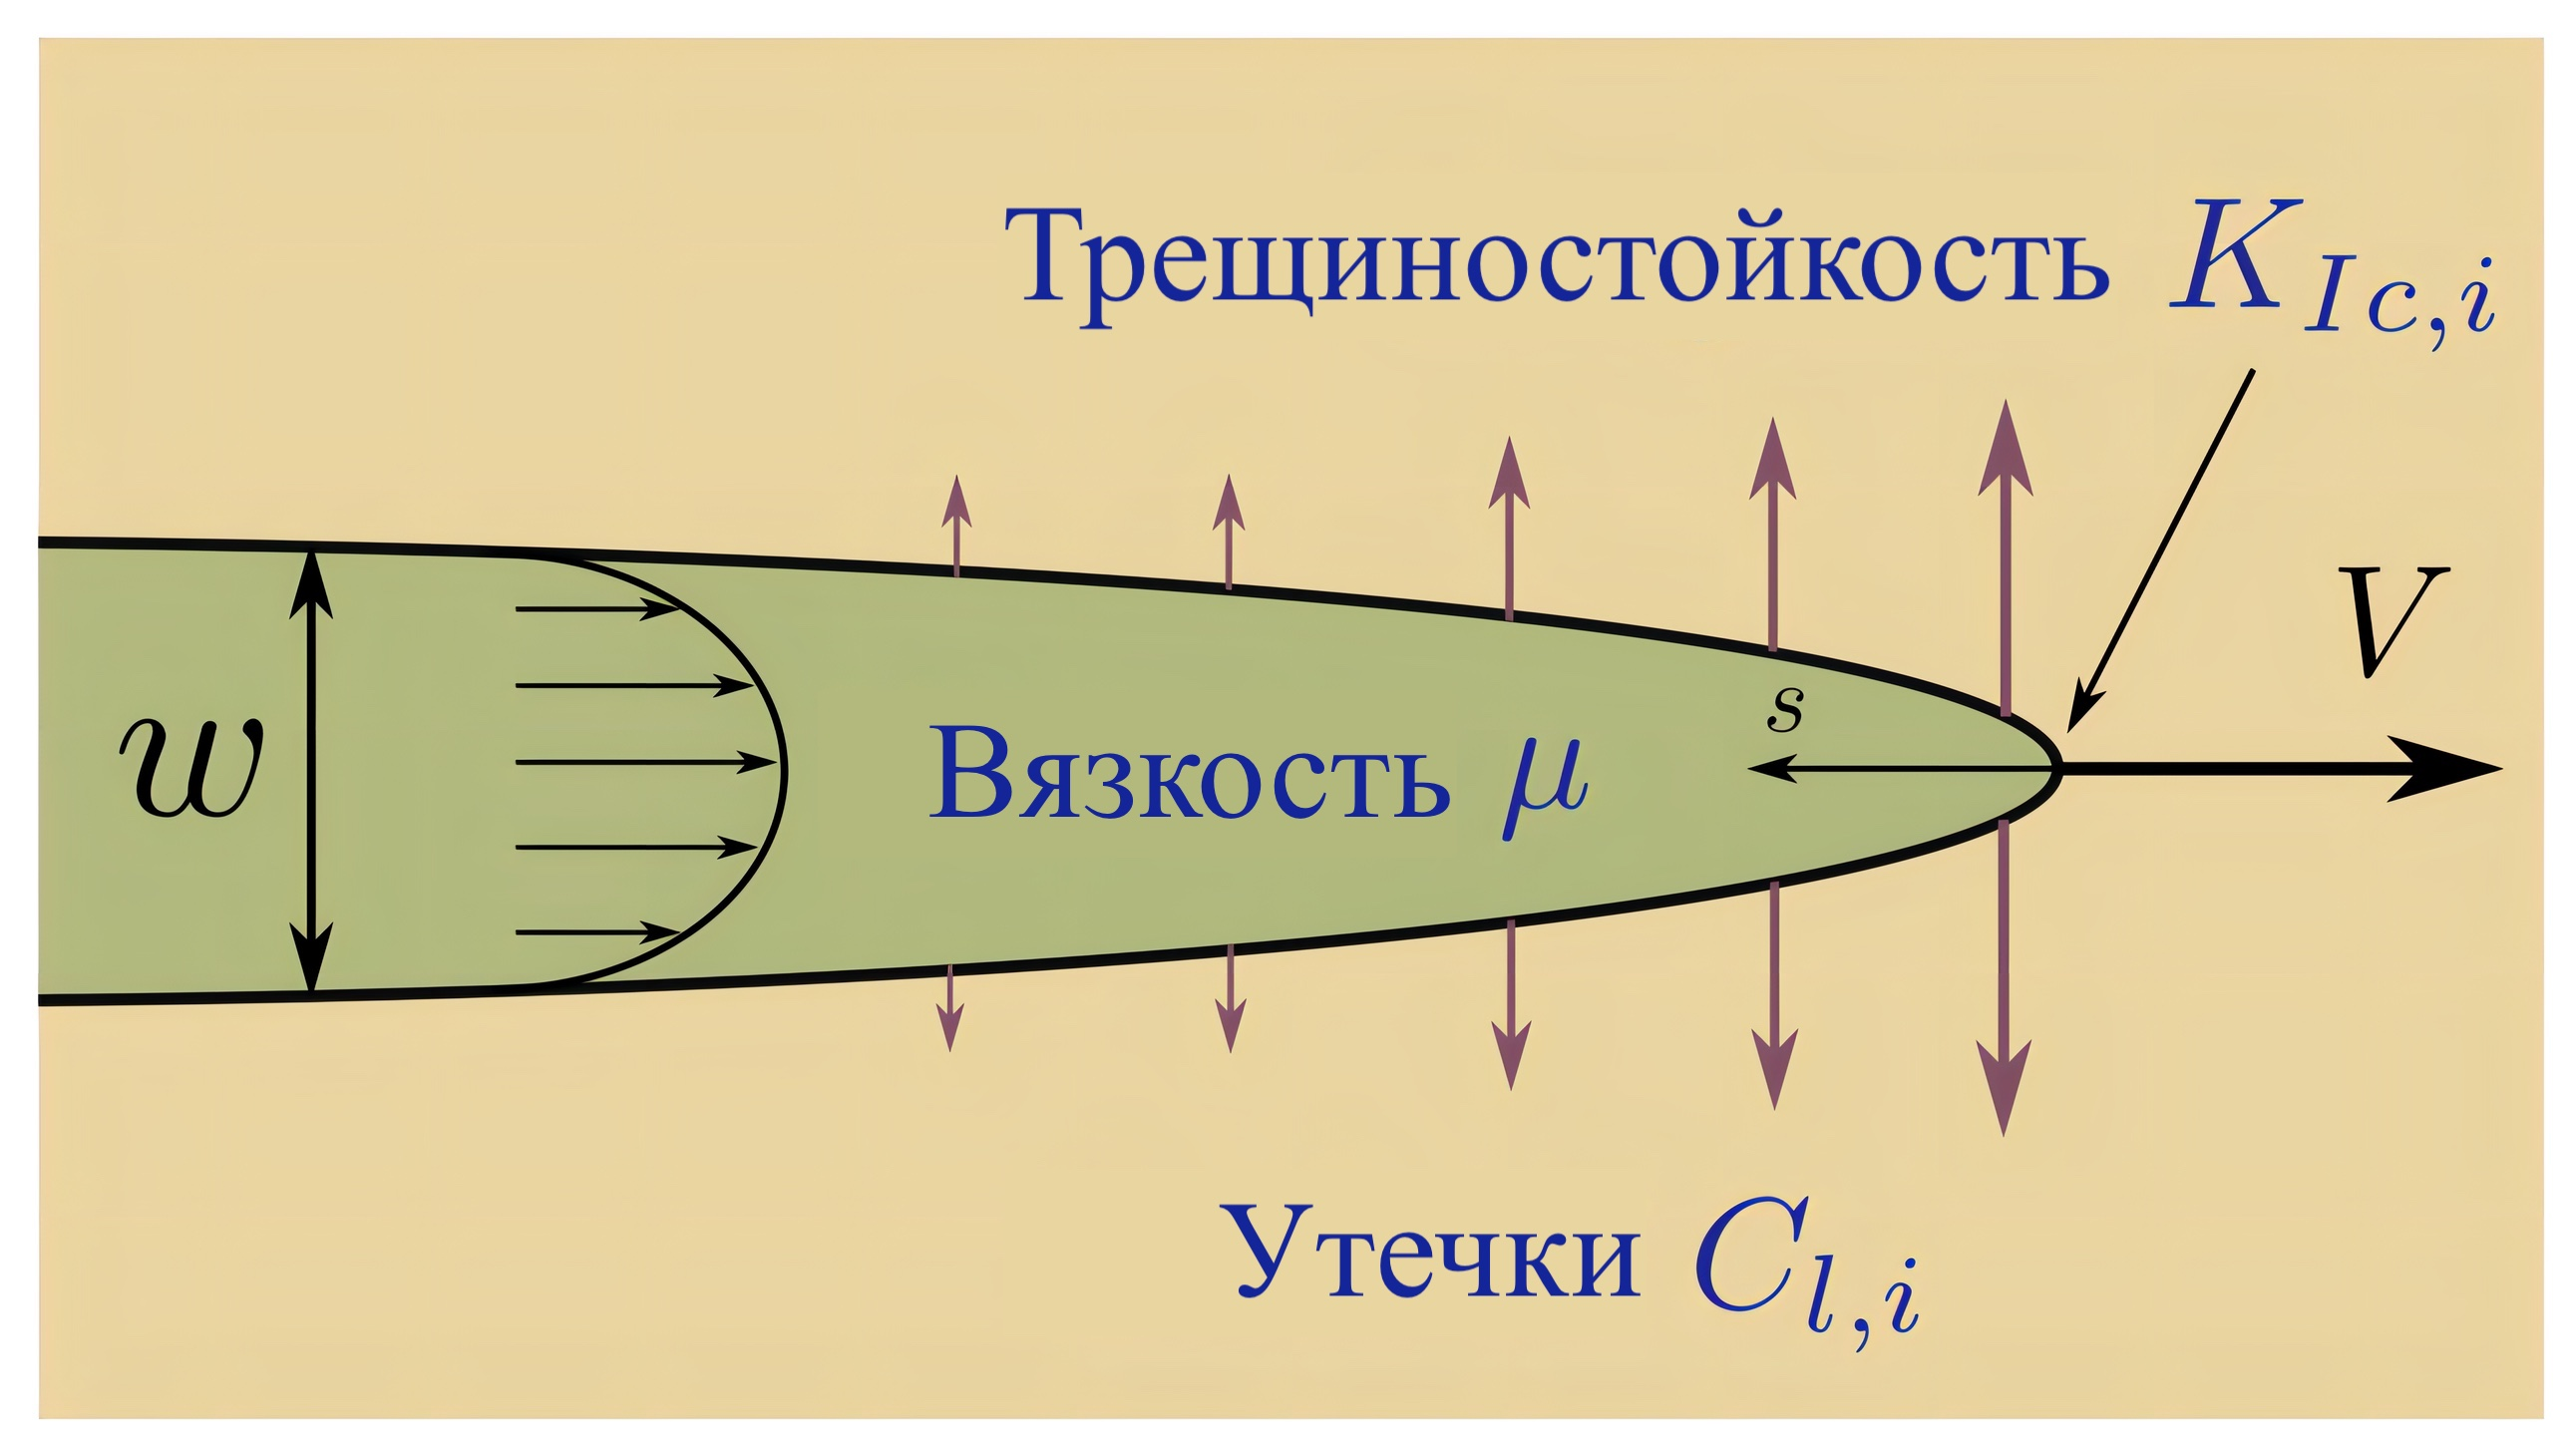
\includegraphics[width=\linewidth]{images/planar3D_tip_model_new.jpg}}\hfill\break\\ \hline
	Pseudo3D&Длина трещины $l(t)$ много больше её высоты $h(x,t)$; высота трещины изменяется как по координате $x$, так и со временем $t$; в каждом вертикальном сечении давление одинаково по сечению (из этого условия следует одномерность течения жидкости в трещине)\break\hfill\break (рисунок заимствован из \cite{dontsov_peirce,baykin_course})&\hfill\break\makecell[c]{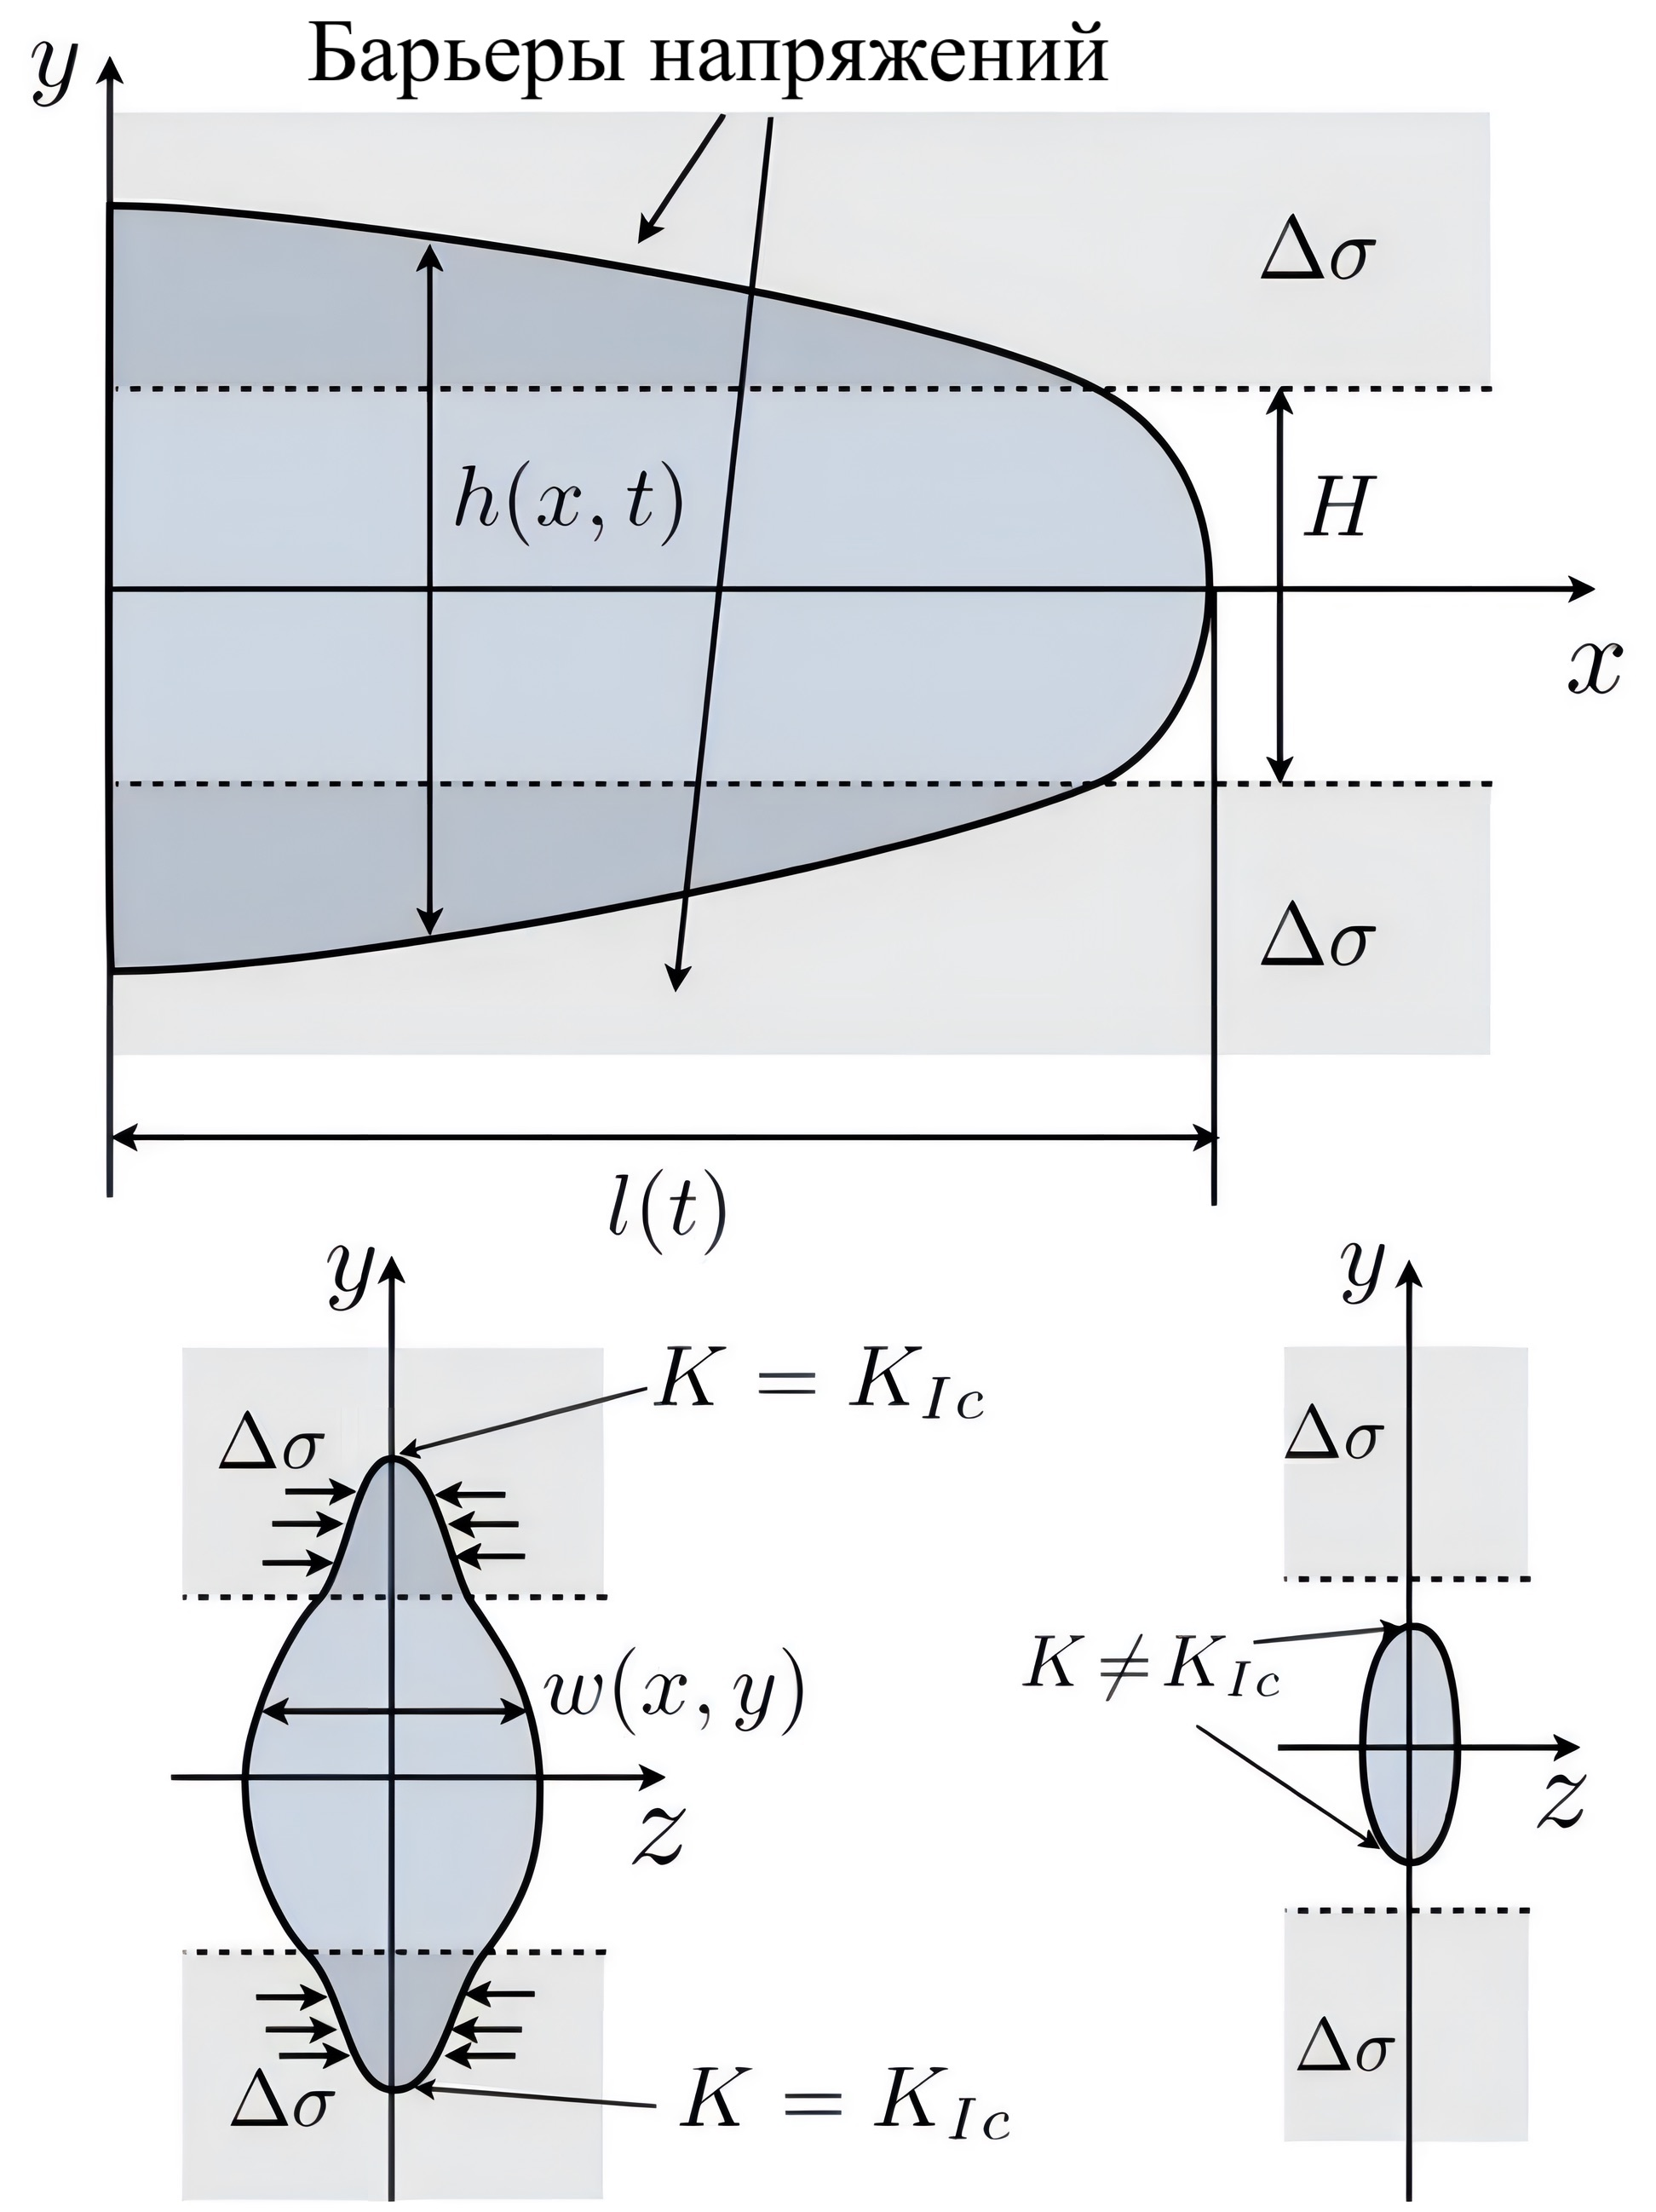
\includegraphics[width=\linewidth]{images/pseudo3D_model_new.jpg}}\hfill\break\\ \hline
	Перкинса- Керна- Нордгрена (модель PKN или модель трещины постоянной высоты)&Длина трещины много больше её фиксированной высоты $H$; в каждом вертикальном сечении давление одинаково по сечению (из этого условия следует эллиптичность вертикального сечения трещины и одномерность течения жидкости в трещине)\break\hfill\break (рисунок заимствован из \cite{adachi})&\hfill\break\makecell[c]{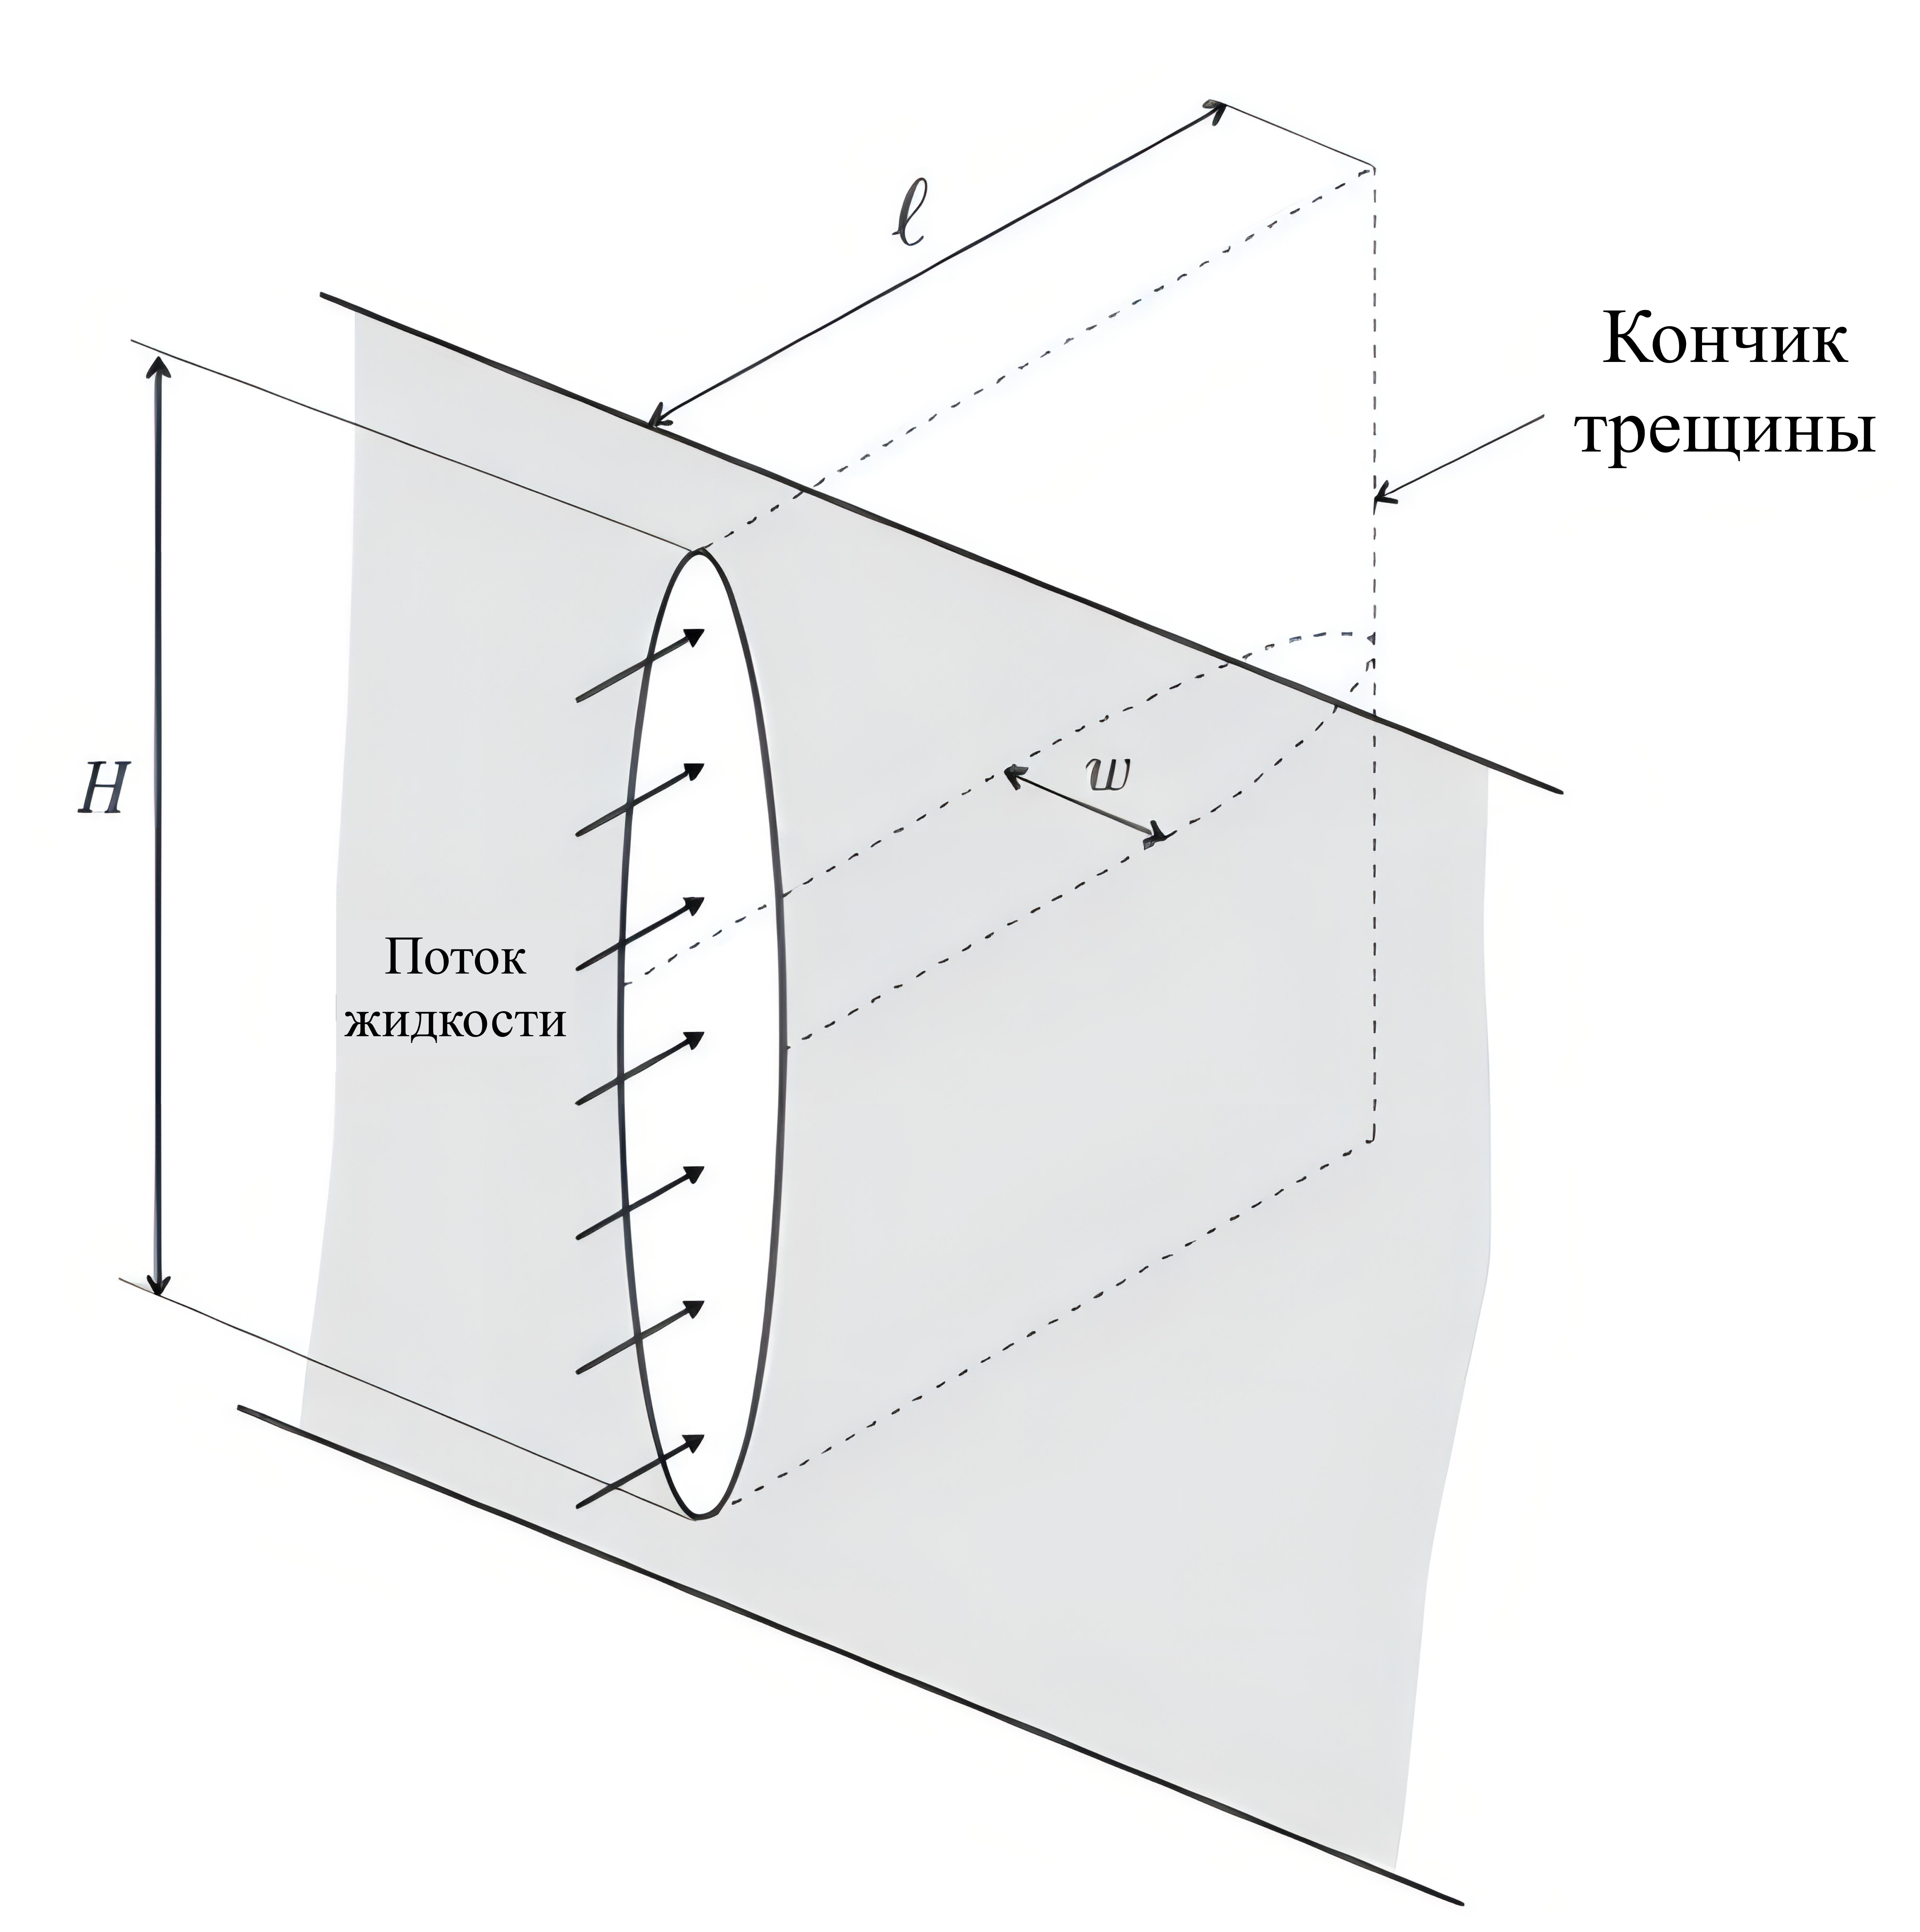
\includegraphics[width=\linewidth]{images/pkn_model_new.jpg}}\hfill\break\\ \hline
	Модель радиальной трещины (или модель трещины в форме копейки)&Точечный или очень короткий перфорированный интервал; бесконечный по всем направлениям однородный пласт; максимальная высота трещины равна её длине\break\hfill\break (рисунок заимствован из \cite{adachi})&\hfill\break\makecell[c]{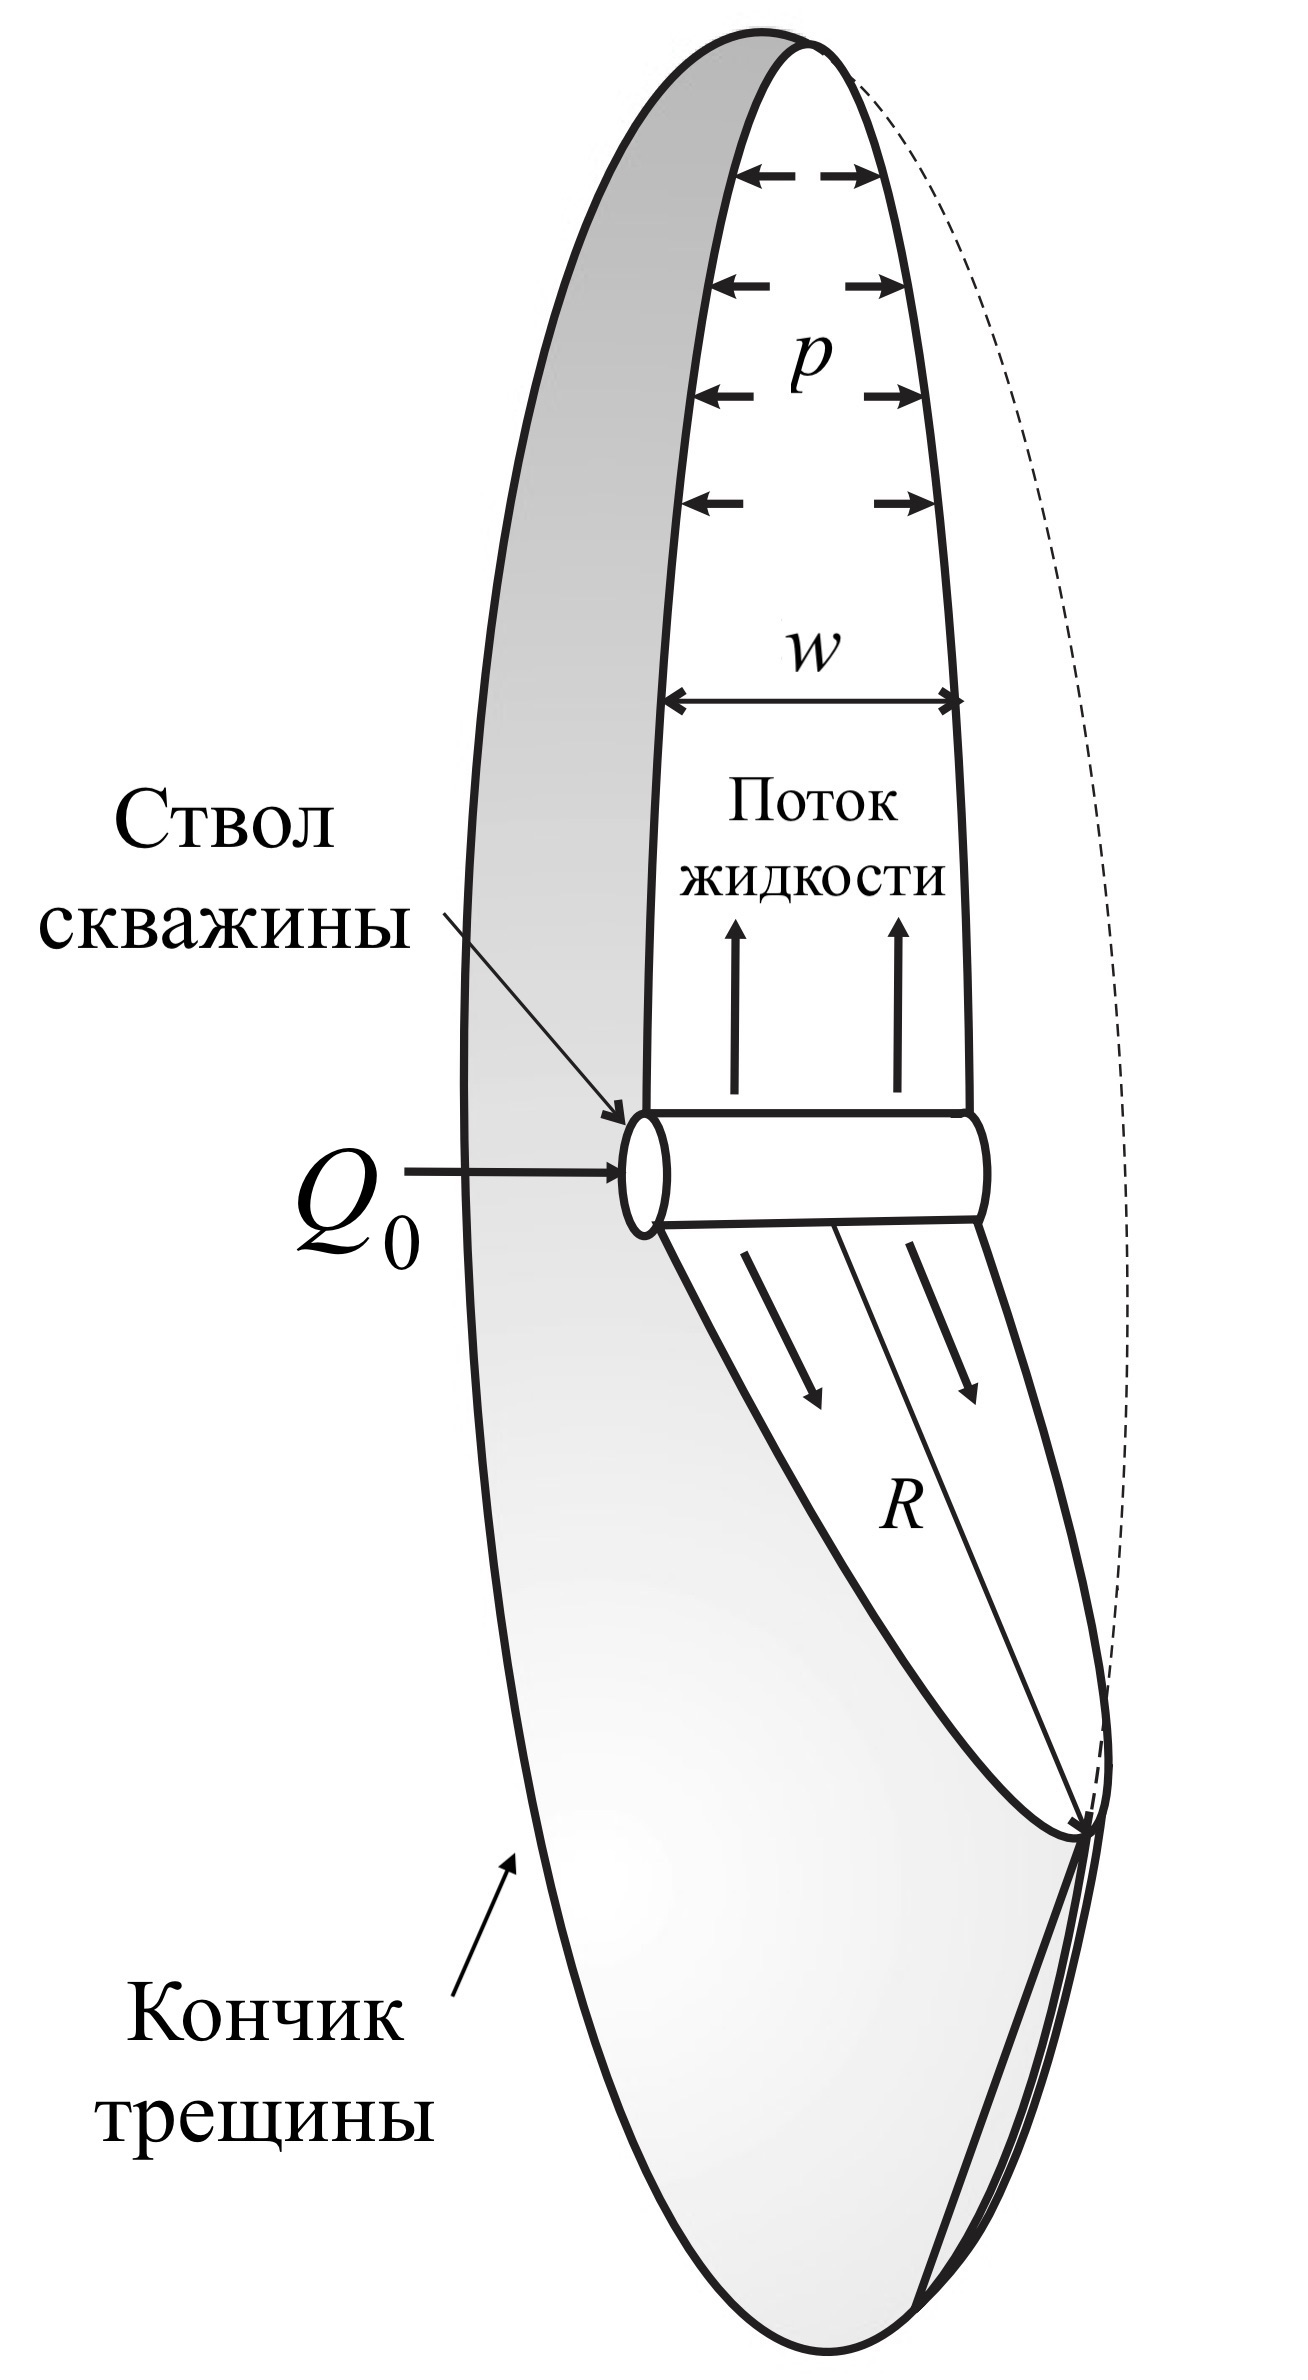
\includegraphics[width=.5\linewidth]{images/radial_model_new_vertical.jpg}}\hfill\break\\ \hline
	Христиано- вича- Желтова- Гиртсма- деКлерка (модель KGD)&Высота трещины много больше её длины; вертикальное сечение трещины прямоугольно; в горизонтальной плоскости выполняется условие плоской деформации\break\hfill\break (рисунок заимствован из \cite{adachi})&\hfill\break\makecell[c]{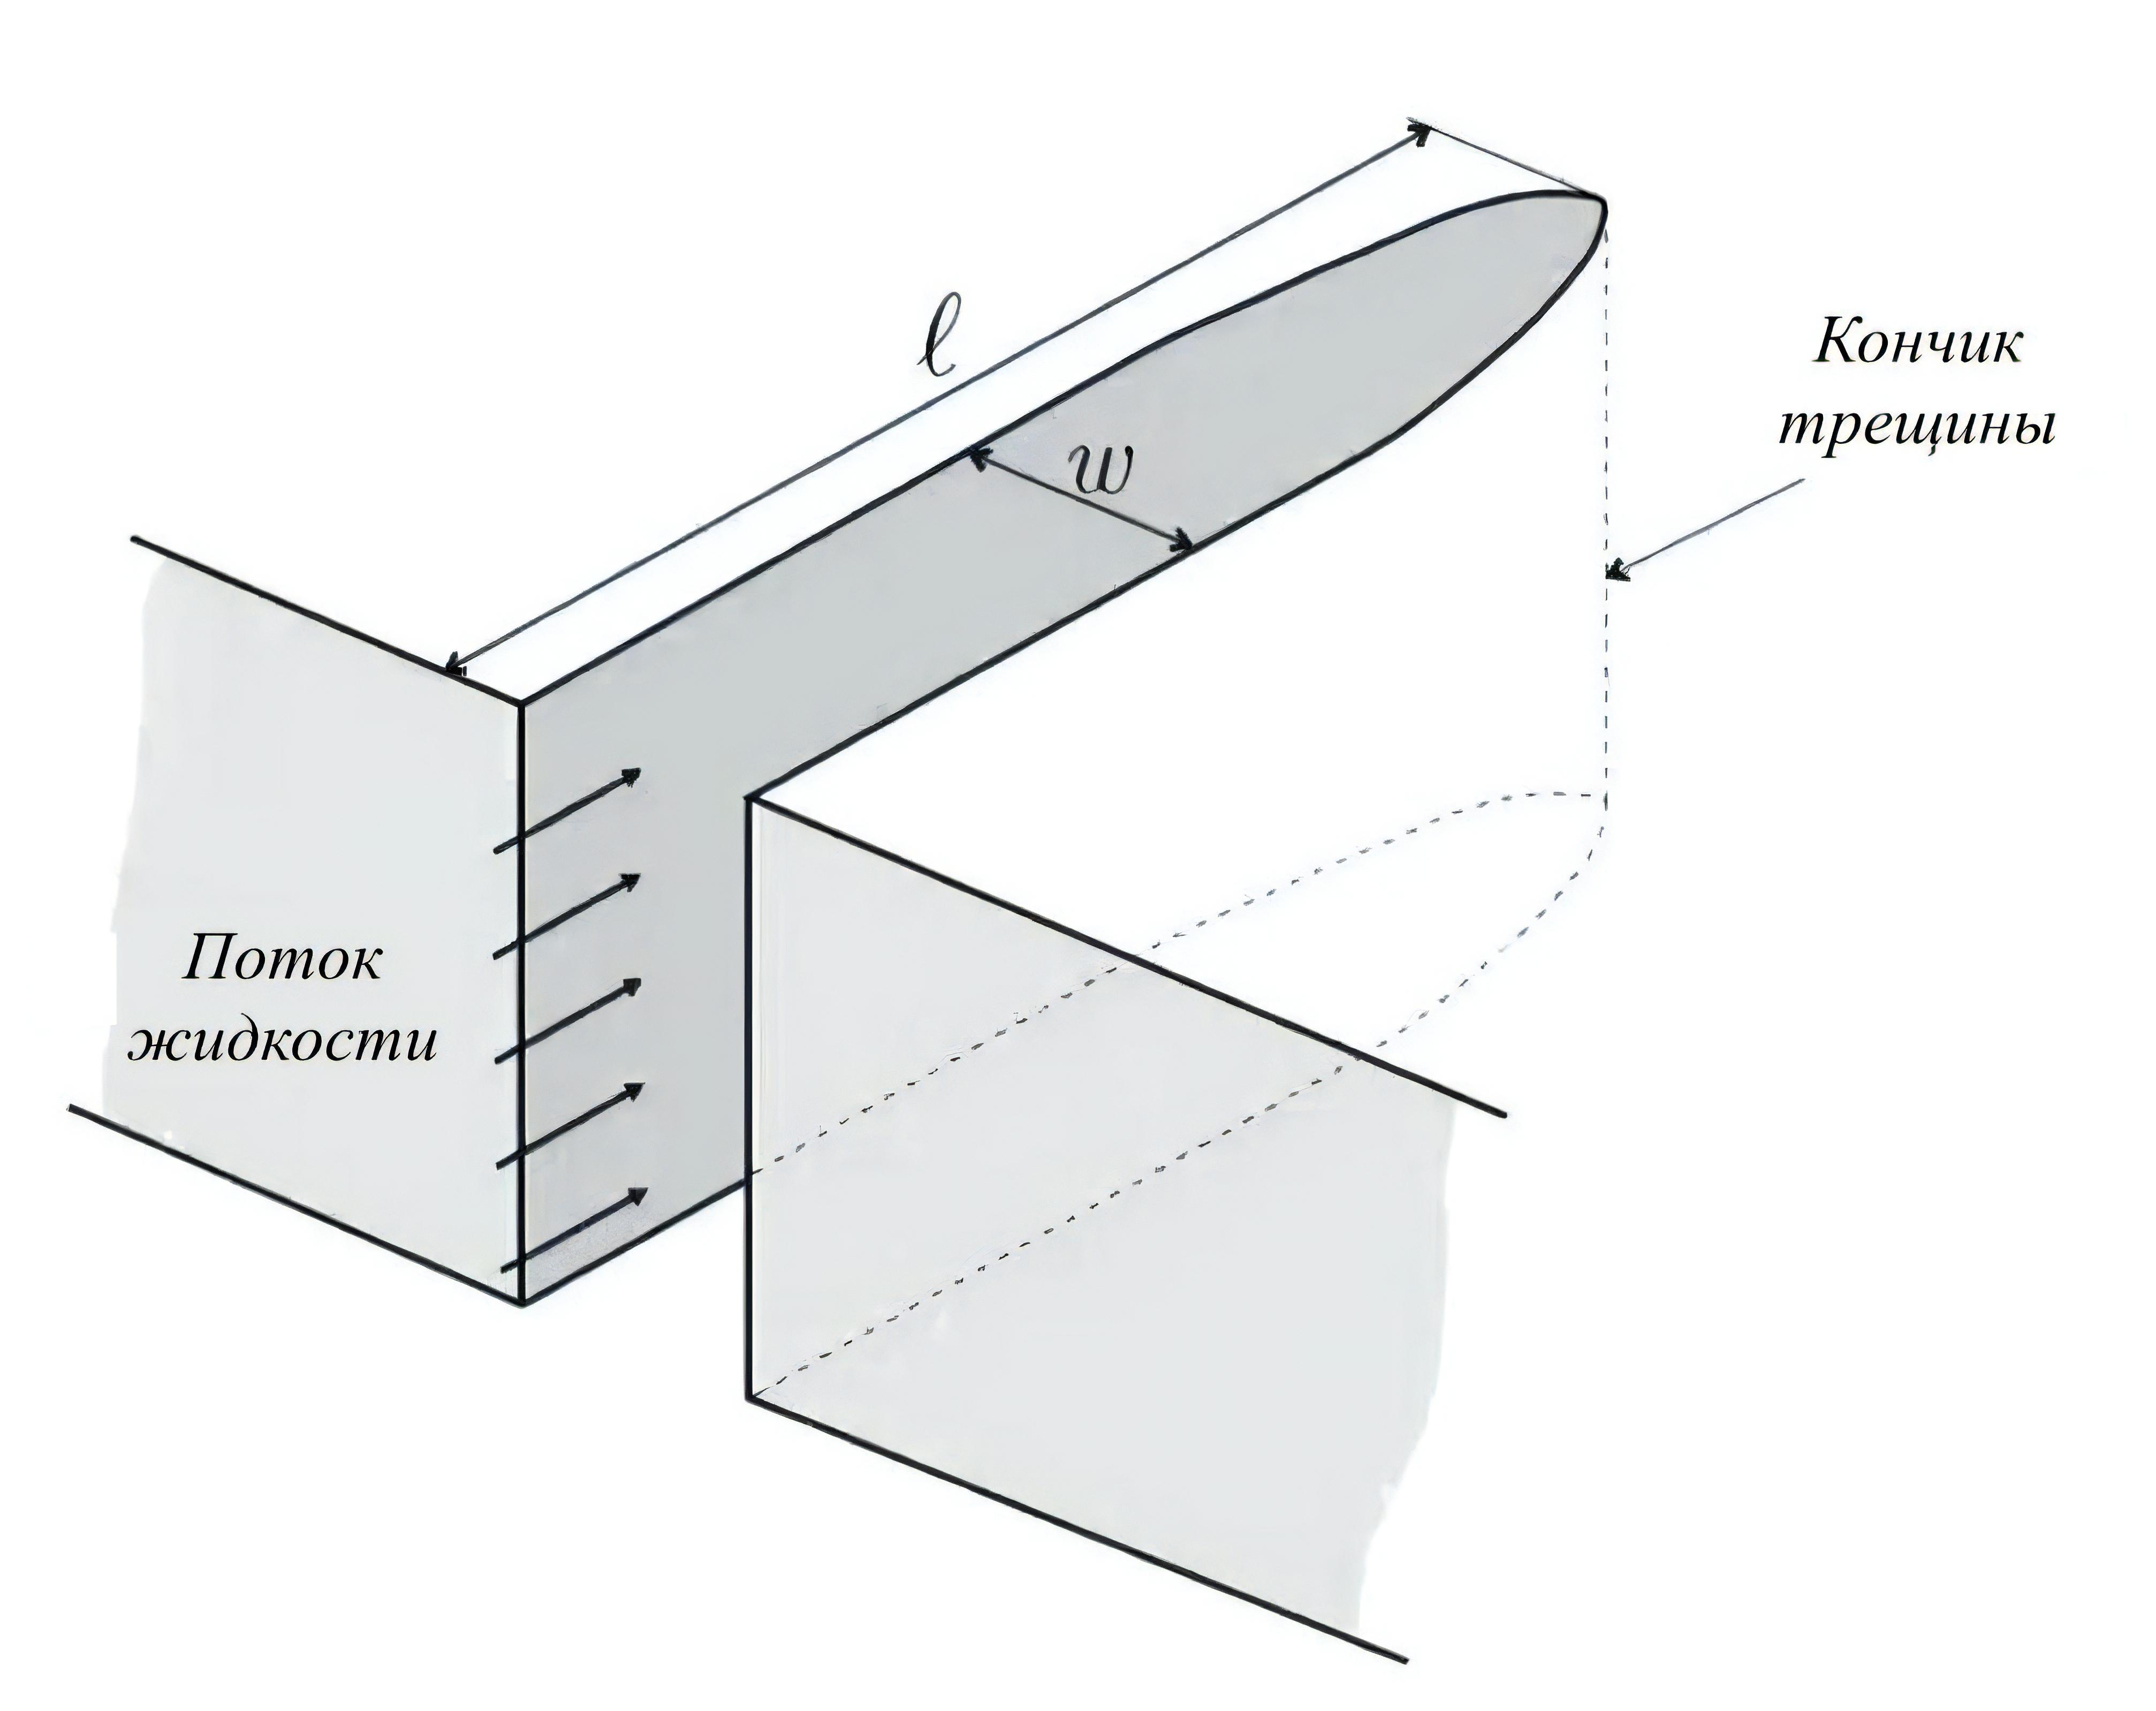
\includegraphics[width=\linewidth]{images/kgd_scheme_better.jpg}}\hfill\break\\ \hline
	
\end{longtable}
\normalsize% возвращаем шрифт к нормальному
\endgroup

Исторически первой С.А.Христиановичем и Ю.П.Желтовым (и независимо от них Гиртсма и деКлерком) в 1955 году была разработана модель KGD \cite{khristianovic_zheltov}, которая хорошо описывает поведение трещины, распространяющейся из протяжённого перфорированного интервала, на ранних временах её распространения.

Также была разработана модель радиальной трещины ГРП, которая реализуется при гидроразрыве относительно мощных однородных пластов из ограниченных (точечных) перфорированных интервалов.
Подробное описание модели радиальной трещины представлено в работах \cite{madyarova,savitski}.

В 1961 году исследователями Перкинсом и Керном была разработана более распространённая модель Перкинса-Керна \cite{perkins_kern}, которая хорошо описывает поведение трещины, распространяющейся из протяжённого перфорированного интервала, на поздних временах её распространения.
В дальнейшем Нордгреном \cite{nordgren} к модели Перкинса-Керна были добавлены эффекты потери жидкости (модель утечек жидкости из трещины).

Любая модель трещины гидроразрыва пласта состоит из нескольких основных компонентов, а именно из:

1) уравнения баланса жидкости с учётом утечек;

2) модели течения жидкости с заданной реологией;

3) уравнения упругости, характеризующего равновесие горной породы;

4) условия распространения трещины;

5) модели транспорта проппанта.

В специфичных случаях некоторые из этих компонент могут не рассматриваться.
Например, при моделировании трещин автоГРП не используется модель транспорта проппанта (так как в трещину закачивается вода) и модель жидкости (так как вязкостью закачиваемой воды обычно пренебрегают).

Далее будут представлены математические модели трещины KGD, радиальной и PKN.

\section{Модель Христиановича-Желтова-Гиртсма-деКлерка (модель KGD)}
\vspace*{-5mm}

В первой модели гидроразрыва пласта \cite{khristianovic_zheltov}, разработанной С.А.Христиановичем и Ю.П.Желтовым, рассматривается трещина одной и той же ширины в любом горизонтальном сечении в пределах фиксированной толщины пласта $h$ (раскрытие трещины не зависит от вертикальной координаты).
Другими словами, используется допущение о плоской деформации в каждой горизонтальной плоскости (это допущение более приемлемо для коротких трещин, у которых $2x_{\!f}\ll h$, где $x_{\!f}$ -- полудлина трещины).
В основе модели лежит физическая гипотеза, что верхняя и нижняя поверхности трещины свободно скользят по кровле и подошве пласта \cite{economides}.

В результате получается трещина прямоугольного вертикального сечения, а ширина трещины рассматривается как функция координаты $x$.

Другими словами, в модели KGD предполагается, что высота трещины $h$ много больше её длины $2x_{\!f}$, у трещины прямоугольное вертикальное сечение и верно допущение о плоской деформации в горизонтальной плоскости.
Эти допущения позволяют свести задачу о моделировании роста трещины к одномерной постановке.


\begin{figure}[H]
	\adjustbox{minipage=1.3em,valign=t}{\subcaption{}\label{fig:kgd-model-3D}}%
	\begin{subfigure}[t]{\dimexpr.5\linewidth-1.3em\relax}
		\centering
		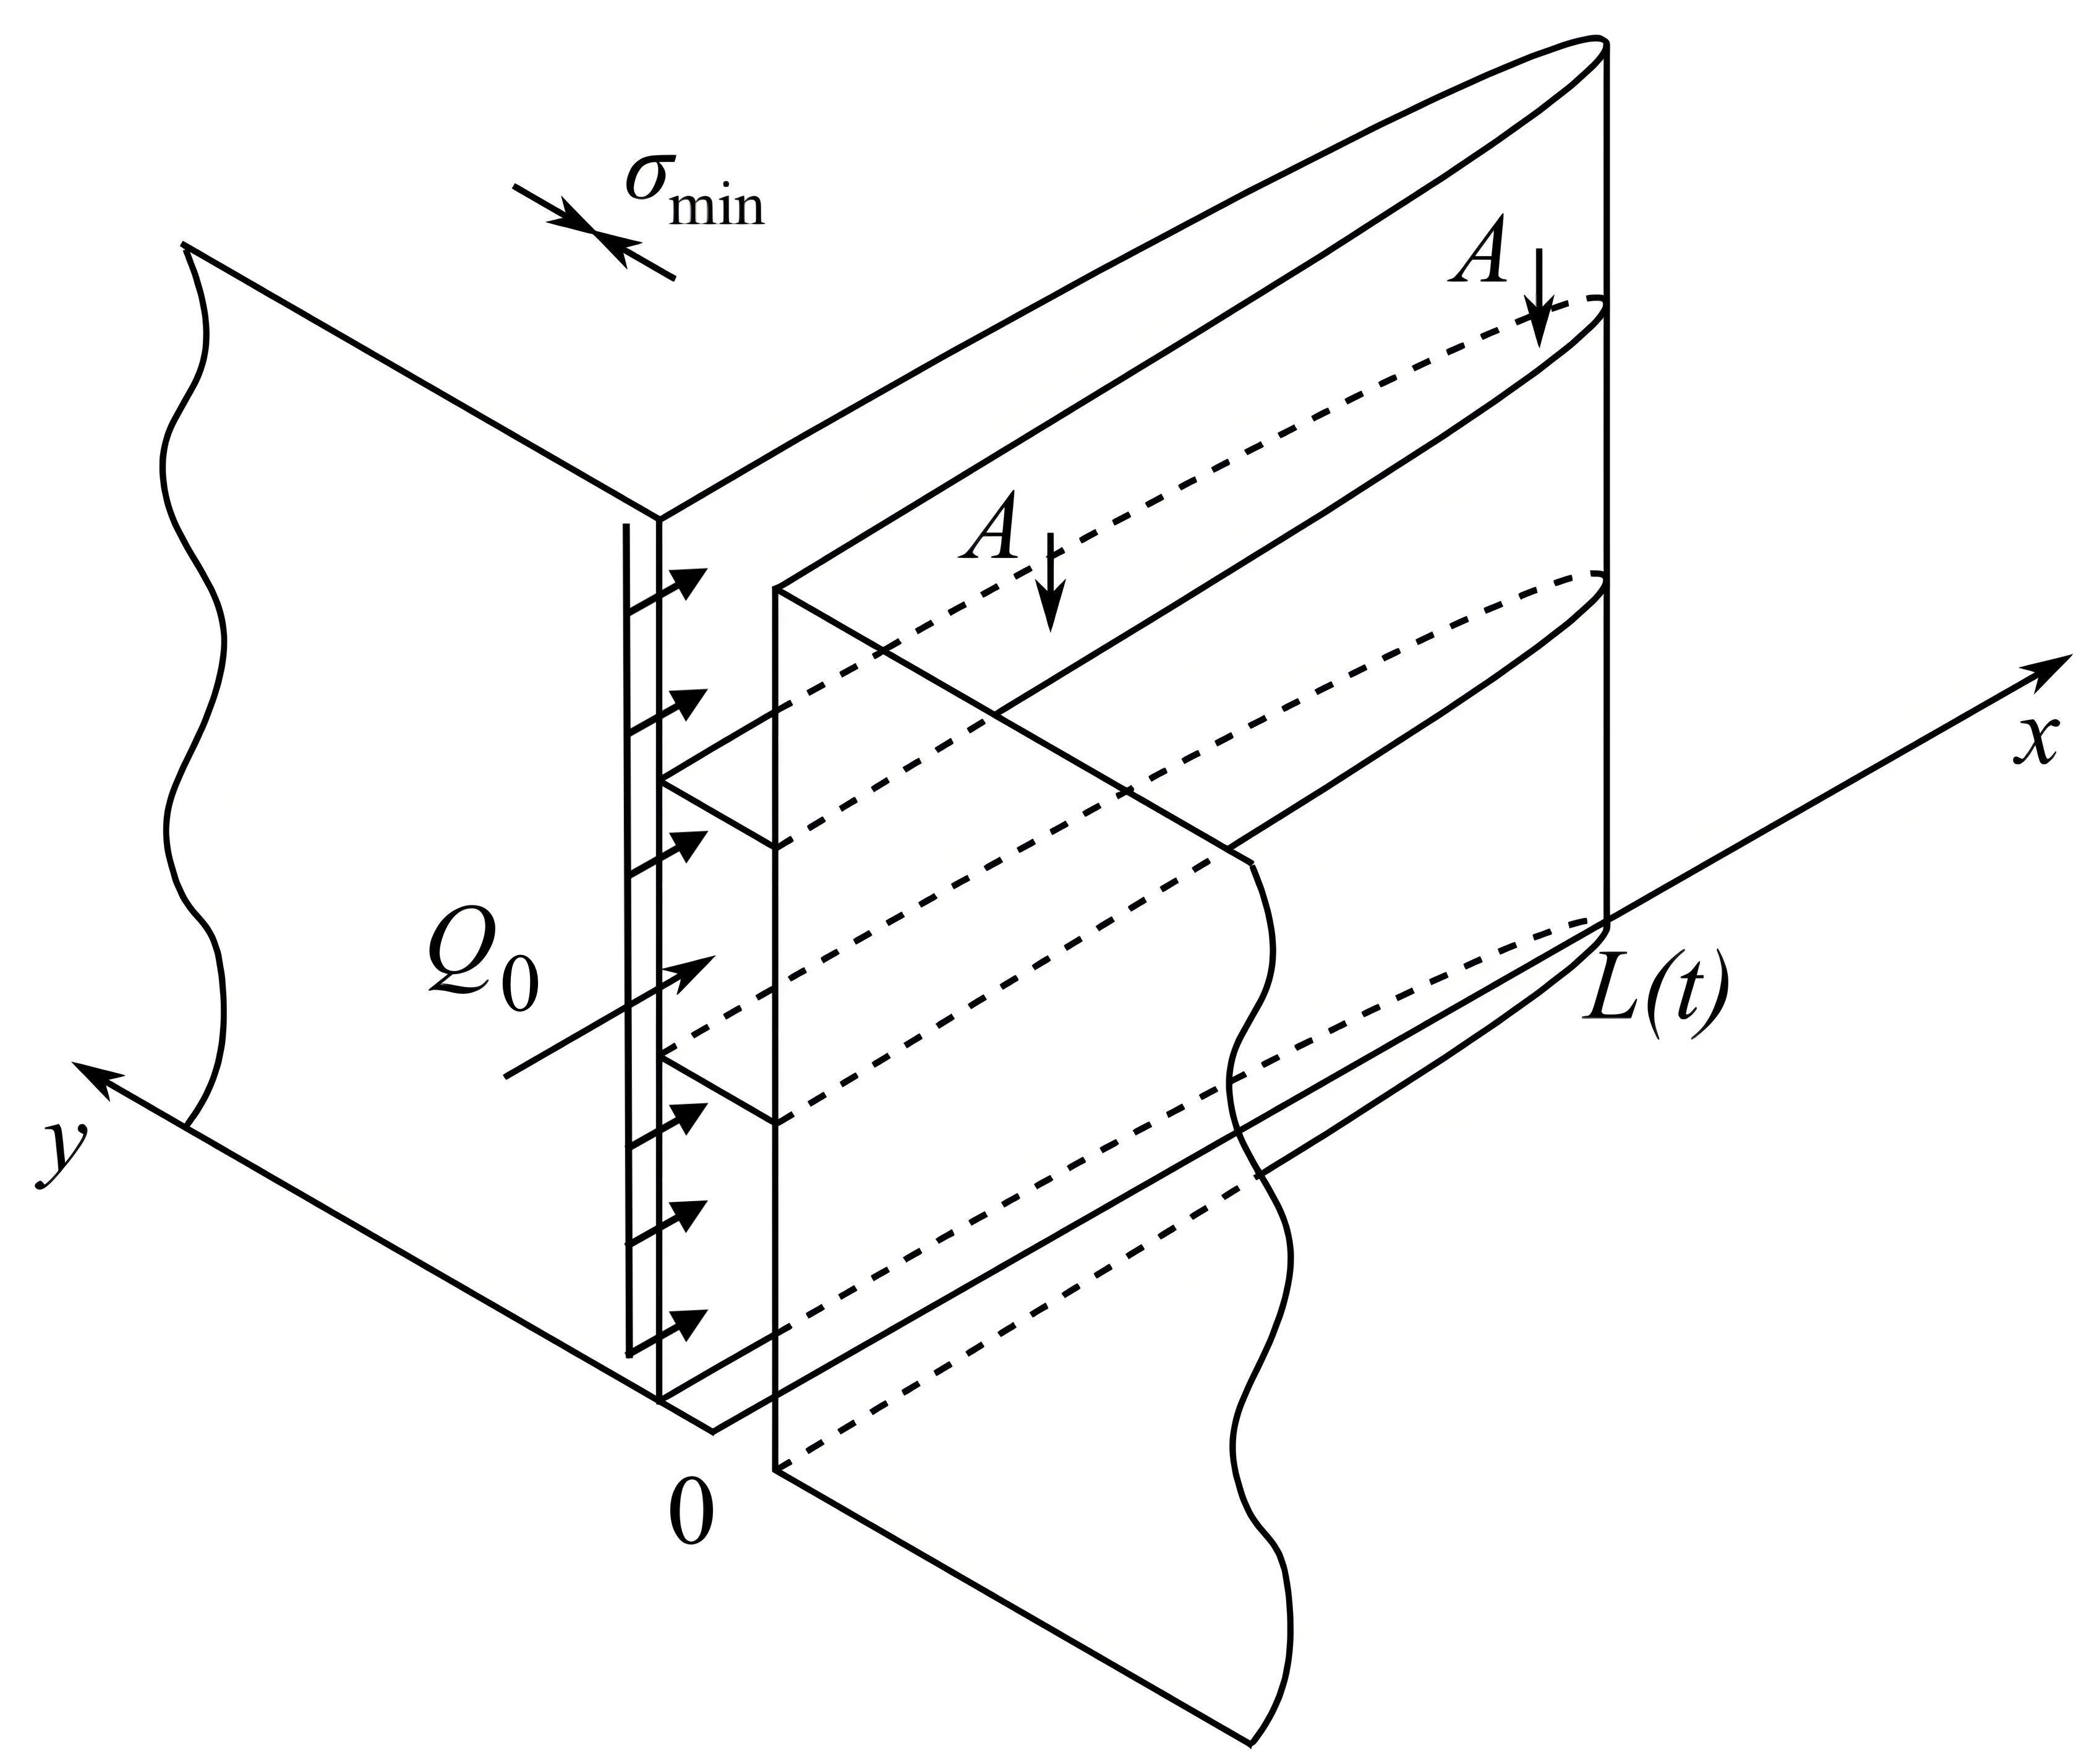
\includegraphics[width=.95\linewidth,valign=t]{images/kgd_model_3D.jpg}
	\end{subfigure}
\hfill %выровнять по ширине
	\adjustbox{minipage=1.3em,valign=t}{\subcaption{}\label{fig:kgd-model-projections}}%
	\begin{subfigure}[t]{\dimexpr.5\linewidth-1.3em\relax}
		\centering
		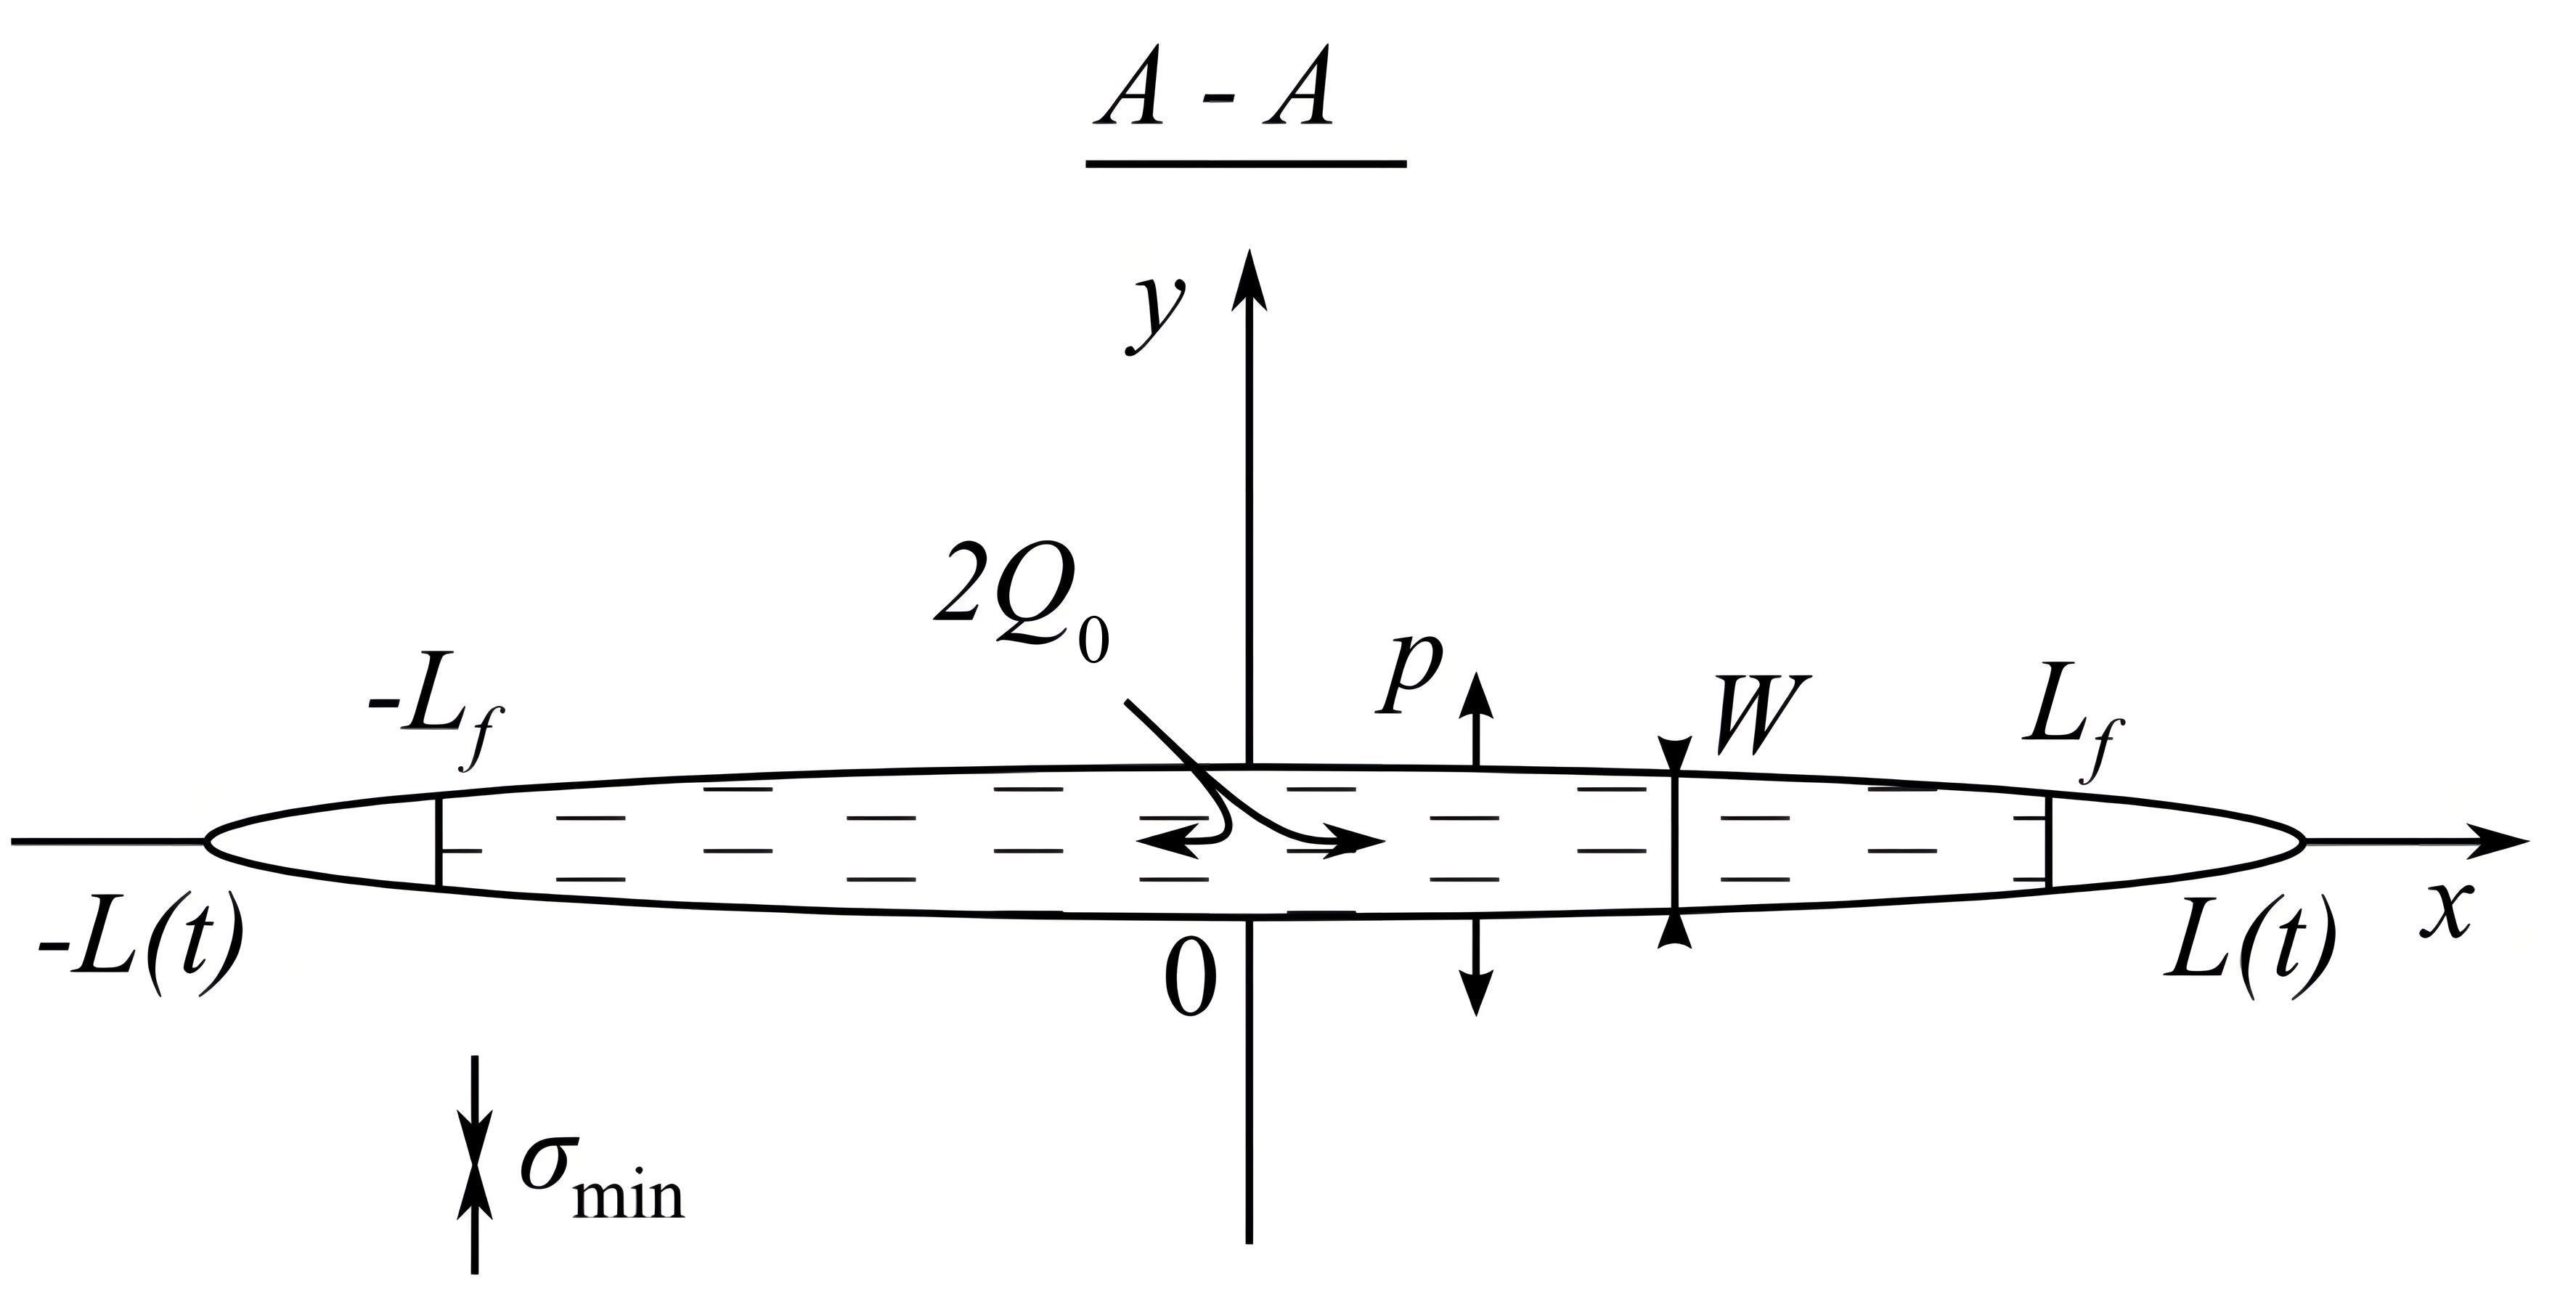
\includegraphics[width=.95\linewidth,valign=t]{images/kgd_model_A-A_plane.jpg}
	\end{subfigure}
\captionsetup{justification=centering} %центрировать
\caption{Геометрия трещины KGD \cite{esipov}: {\itshape a} --- в 3D; {\itshape b} --- проекция A-A} 
\label{fig:kgd-model}
\end{figure}

\textbf{Уравнение баланса жидкости.}

Для трещины KGD верно равенство, выражающее закон сохранения объёма жидкости в малом выделенном объёме трещины:
\beq
w(t+dt)dx = w(t)dx+q_x(x)dt-q_x(x+dx)dt-2gdxdt,
\eeq
где $w$ -- раскрытие выделенного объёма трещины,
$q_x$ -- поток жидкости вдоль оси $Ox$,
$g$ -- скорость утечек.

Откуда получаем уравнение баланса жидкости:
\beq
\frac{\partial w}{\partial t}+\frac{\partial q_x}{\partial x}+2g=Q_0(t)\delta(x),
\eeq
где $g$ -- скорость утечек из трещины в пласт;
$Q_0(t)$ -- расход жидкости на скважине (в м$^2$/с, чтобы размерности были согласованы -- как бы закачиваем жидкость в трещину на плоскости, поэтому метры в квадрате, а не в кубе);
$\delta(x)$ -- дельта-функция Дирака.

Из модели Картера \cite{karter} скорость утечек:
\beq
g=\frac{C_l}{\sqrt{t-t_0(x)}},
\eeq
где $C_l$ -- коэффициент утечек Картера;
$t_0(x)$ -- время, за которое фронт трещины достигнет координаты $x$.

Таким образом, уравнение баланса жидкости с учётом утечек для трещины KGD запишется в следующей форме:
\beq
\frac{\partial w}{\partial t}+\frac{\partial q}{\partial x}+\frac{C'}{\sqrt{t-t_0(x)}}=Q_0(t)\delta(x),
\eeq
где $C'=2C_l$ -- масштабированный коэффициент утечек Картера.\\

\textbf{Модель течения жидкости.}

В модели трещины KGD рассматривается одномерное течение жидкости вдоль трещины, то есть имеется только одна компонента вектора скорости, которая изменяется в зависимости от координаты $y$:
\beq
v=v_x(y)
\eeq
Из уравнений Навье-Стокса для вязкой ньютоновской жидкости:
\beq\label{Navie_part}
\frac{\partial p}{\partial x}=\frac{\partial\tau}{\partial y}
\eeq
Для ньютоновской жидкости сдвиговое напряжение:
\beq\label{Newton_shear}
\tau = \mu\frac{\partial v}{\partial y}
\eeq
Дополнительно ставим условие прилипания (отсутствия проскальзывания) на границах трещины:
\beq\label{Cave_Boundary}
v|_{y=\pm w/2}=0
\eeq
Общее решение уравнения \eqref{Navie_part} после подстановки \eqref{Newton_shear} запишется в виде:
\beq
v(y)=\frac{\partial p}{\partial x}\frac{y^2}{2}+Ay+B
\eeq
Решение после учёта граничных условий \eqref{Cave_Boundary}:
\beq
v(y)=-\frac{\partial p}{\partial x}\frac{w^2-4y^2}{8\mu}\text{ (течение Пуазейля).}
\eeq
Суммарный поток (расход) жидкости:
\beq
q=\int\limits_{-w/2}^{w/2}v(y)dy=-\frac{w^3}{12\mu}\frac{\partial p}{\partial x}
\eeq

\textbf{Уравнение упругости.}

Упругое равновесие горной породы характеризуется уравнением упругости, которое для трещины KGD запишется в следующей форме \cite{crouch}:
\beq
p(x,t)=\sigma_0-\frac{E'}{4\pi}\int\limits_{-l}^{l}{\frac{w(s)ds}{(x-s)^2}},
\vspace*{-3mm}
\eeq
где $E'=\dfrac{E}{1-\nu^2}$ -- модуль плоской деформации породы; $\sigma_0$ -- минимальное горизонтальное напряжение в пласте.\\

\textbf{Условие распространения.}

Условие распространения трещины KGD в рамках линейно-упругой механики разрушения (ЛУМР) \cite{cherepanov,rice} можно представить в виде:
\beq
\lim_{x\to L}\frac{w}{(L-x)^{1/2}}=
\begin{cases}
\dfrac{K'_{Ic}}{E'},\text{ если }v>0\\[15pt]
\dfrac{K_I'}{E'},\text{ если }v=0
\end{cases},
\eeq
где $K'_{I}=8K_{I}/\sqrt{2\pi}$ -- масштабированный коэффициент интенсивности напряжений;\newline
$K'_{Ic}=8K_{Ic}/\sqrt{2\pi}$ -- масштабированный критический коэффициент интенсивности напряжений, при котором трещина распространяется (масштабированная трещиностойкость породы).

Далее в текущей главе везде будет предполагаться, что $v>0$ (т.е. трещина распространяется) и условие распространения будет записываться через трещиностойкость породы $K_{Ic}$.\\

\textbf{Система уравнений модели KGD.}

Таким образом, система уравнений модели трещины KGD запишется в следующем виде:
\beq\label{PlaneFractureSystem}
\begin{cases}
\dfrac{\partial w}{\partial t}+\dfrac{\partial q}{\partial x}+\dfrac{C'}{\sqrt{t-t_0(x)}}=Q_0(t)\delta(x),\\[15pt]
q=-\dfrac{w^3}{\mu'}\dfrac{\partial p}{\partial x},\\[5pt]
p(x,t)=\sigma_0-\dfrac{E'}{4\pi}\displaystyle\int\limits_{-L(t)}^{L(t)}\dfrac{w(s)ds}{(x-s)^2},\\[20pt]
\displaystyle\lim_{x\to L}\dfrac{w}{(L-x)^{1/2}}=\dfrac{K'}{E'},
\end{cases}
\eeq
где $C'=2C_l$, $\,\,\,\mu'=12\mu$, $\,\,\,E'=\dfrac{E}{1-\nu^2}$, $\,\,\,K'=\dfrac{8K_{Ic}}{\sqrt{2\pi}}$.
\\

Приближённые полуаналитические решения для модели Христиановича-
Желтова-Гиртсма-деКлерка в общем случае и точные аналитические решения в предельных режимах распространения (например, в режиме доминирования трещиностойкости и больших утечках) представлены в работе \cite{dontsov1}.

Стоит упомянуть, что существуют многочисленные расширения модели кончика плоской трещины (в этом случае рассматривается только область вблизи кончика плоской трещины в предположении полубесконечной трещины \cite{baykin_course}; отличается от модели \eqref{PlaneFractureSystem}), в которых рассматриваются жидкости со степенной реологией \cite{dontsov_kresse}, жидкости Гершеля-Балкли \cite{bessmertnykh}, жидкости Карро \cite{moukhtari}, эффект отставания фронта жидкости от фронта трещины \cite{garagash}, эффект турбулентного течения \cite{dontsov_turbulent} и эффект утечек жидкости, зависящих от давления \cite{kanin}.

\section{Модель радиальной трещины ГРП}
\vspace*{-5mm}

\begin{figure}[H]
	\adjustbox{minipage=1.3em,valign=t}{\subcaption{}\label{fig:radial-model-3D}}%
	\begin{subfigure}[t]{\dimexpr.5\linewidth-1.3em\relax}
		\centering
		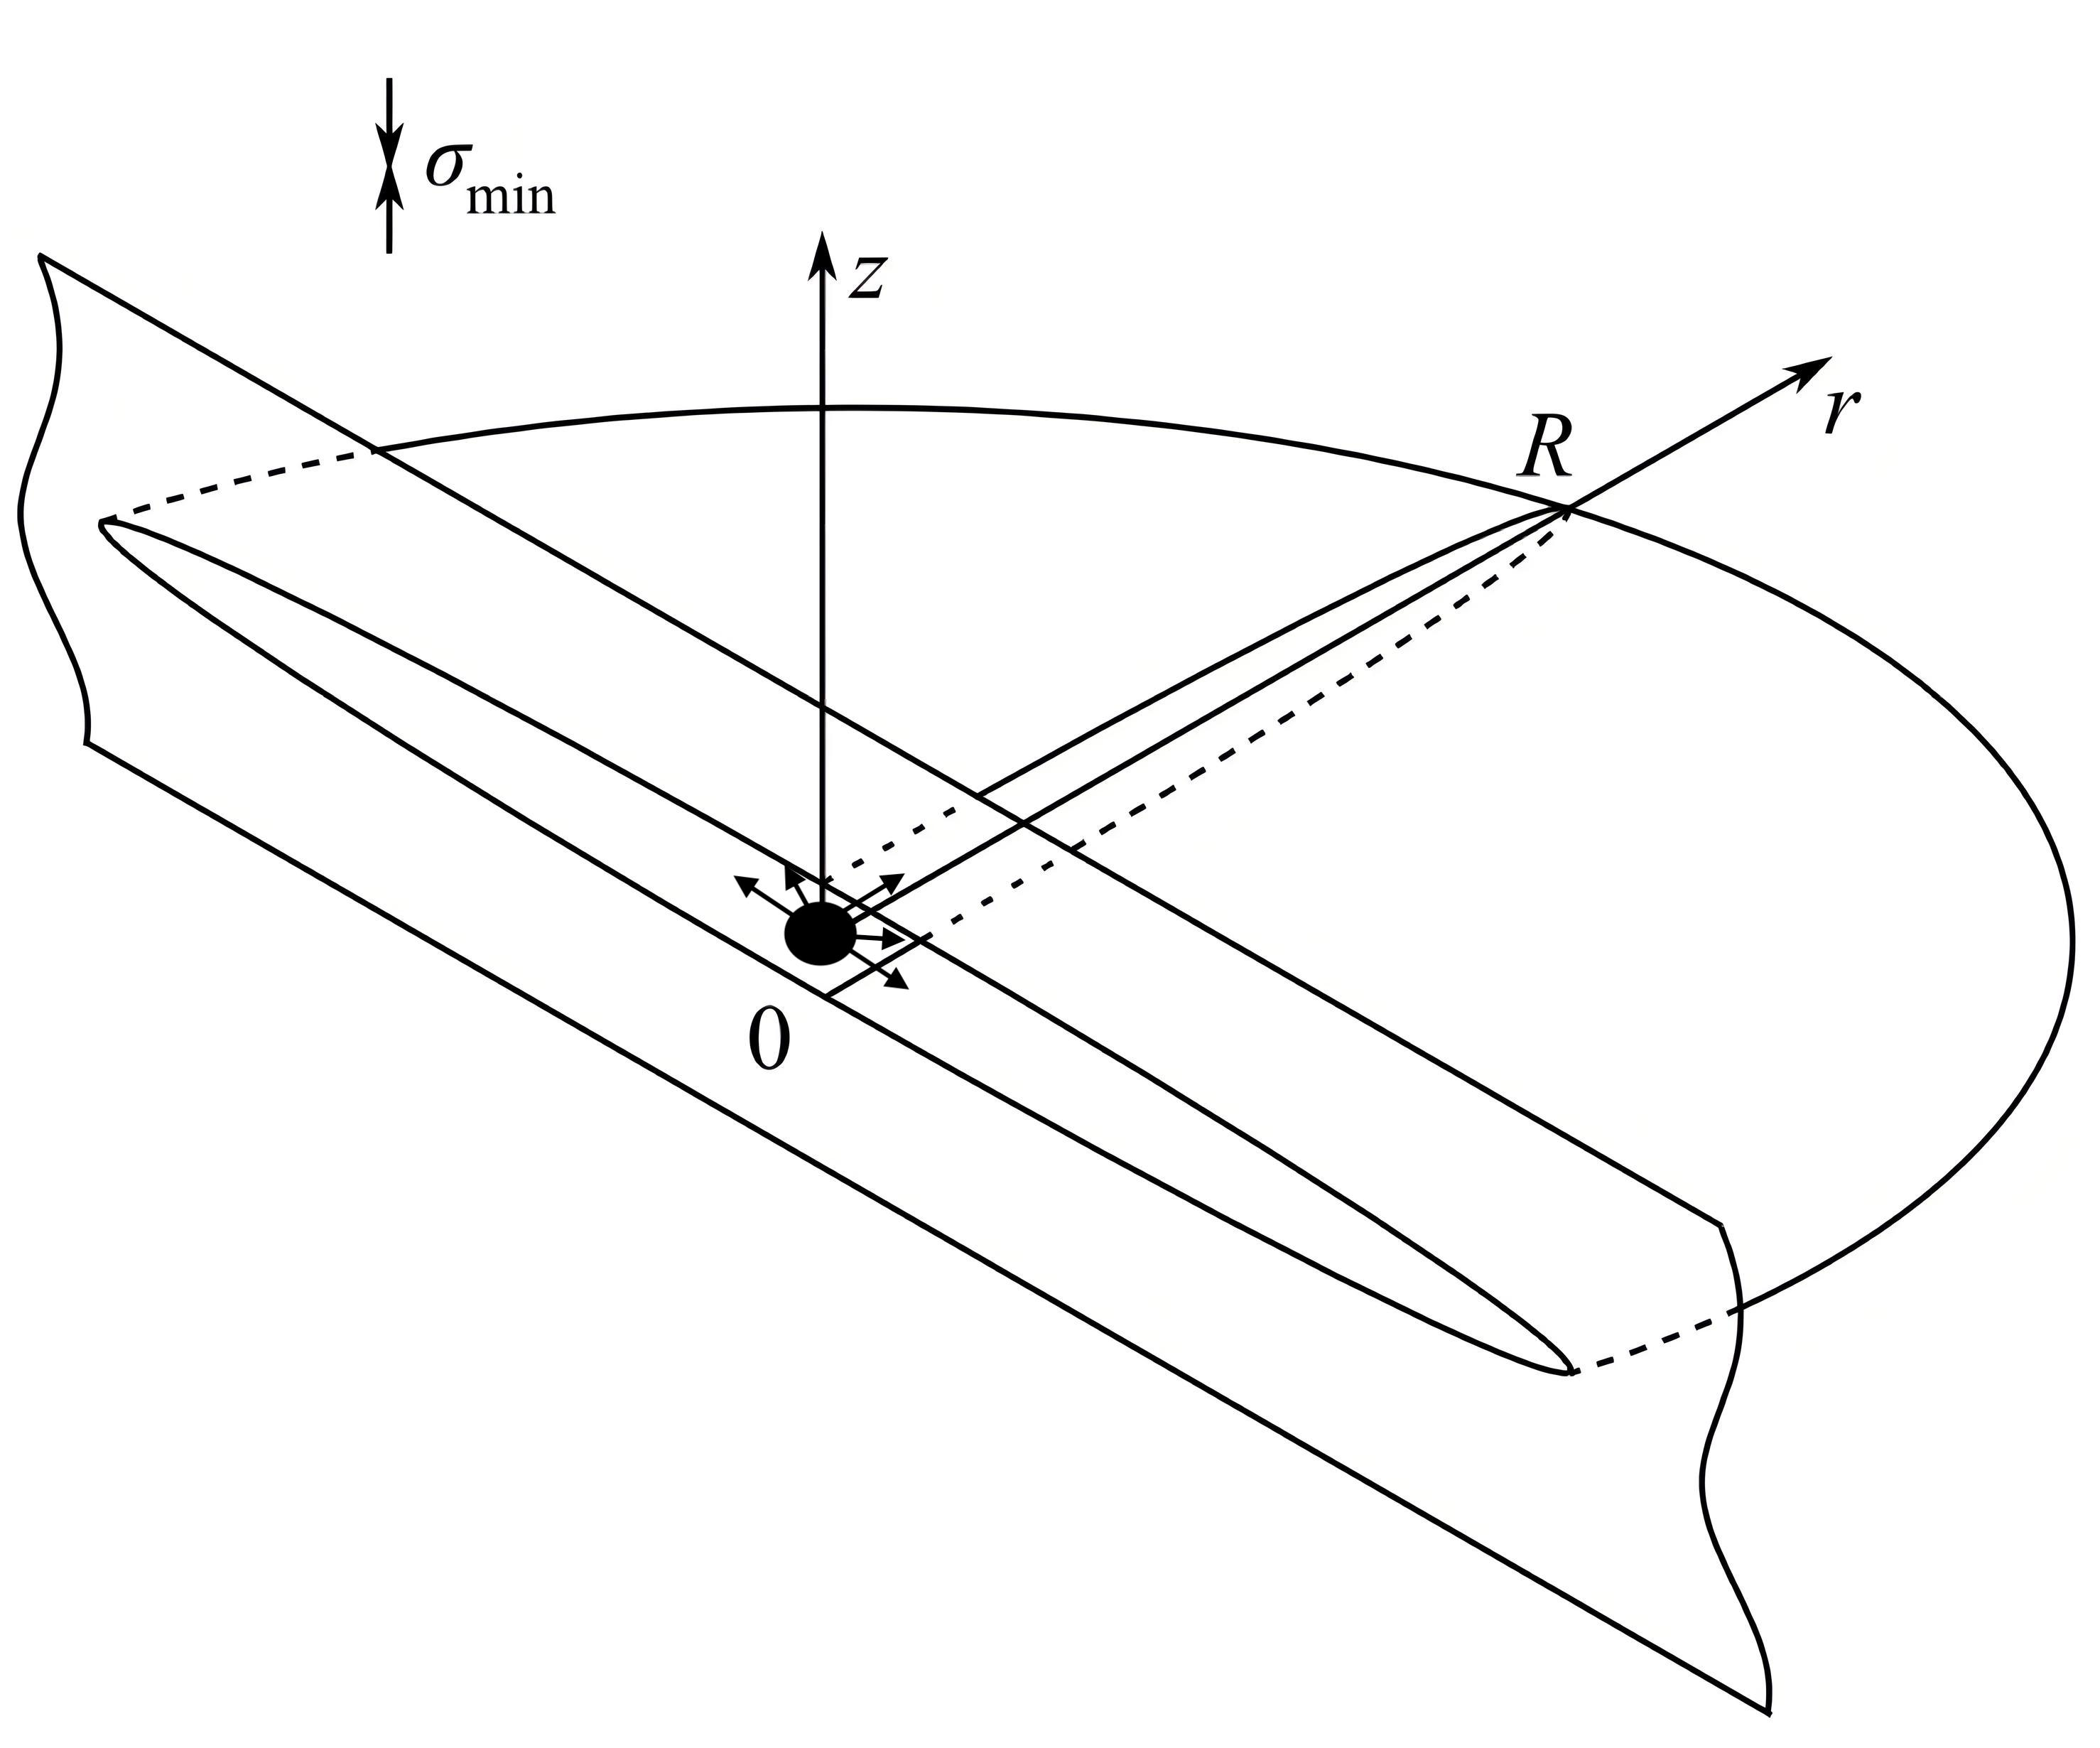
\includegraphics[width=.95\linewidth,valign=t]{images/radial_model_3D.jpg}
	\end{subfigure}
\hfill %выровнять по ширине
	\adjustbox{minipage=1.3em,valign=t}{\subcaption{}\label{fig:radial-model-projections}}%
	\begin{subfigure}[t]{\dimexpr.5\linewidth-1.3em\relax}
		\centering
		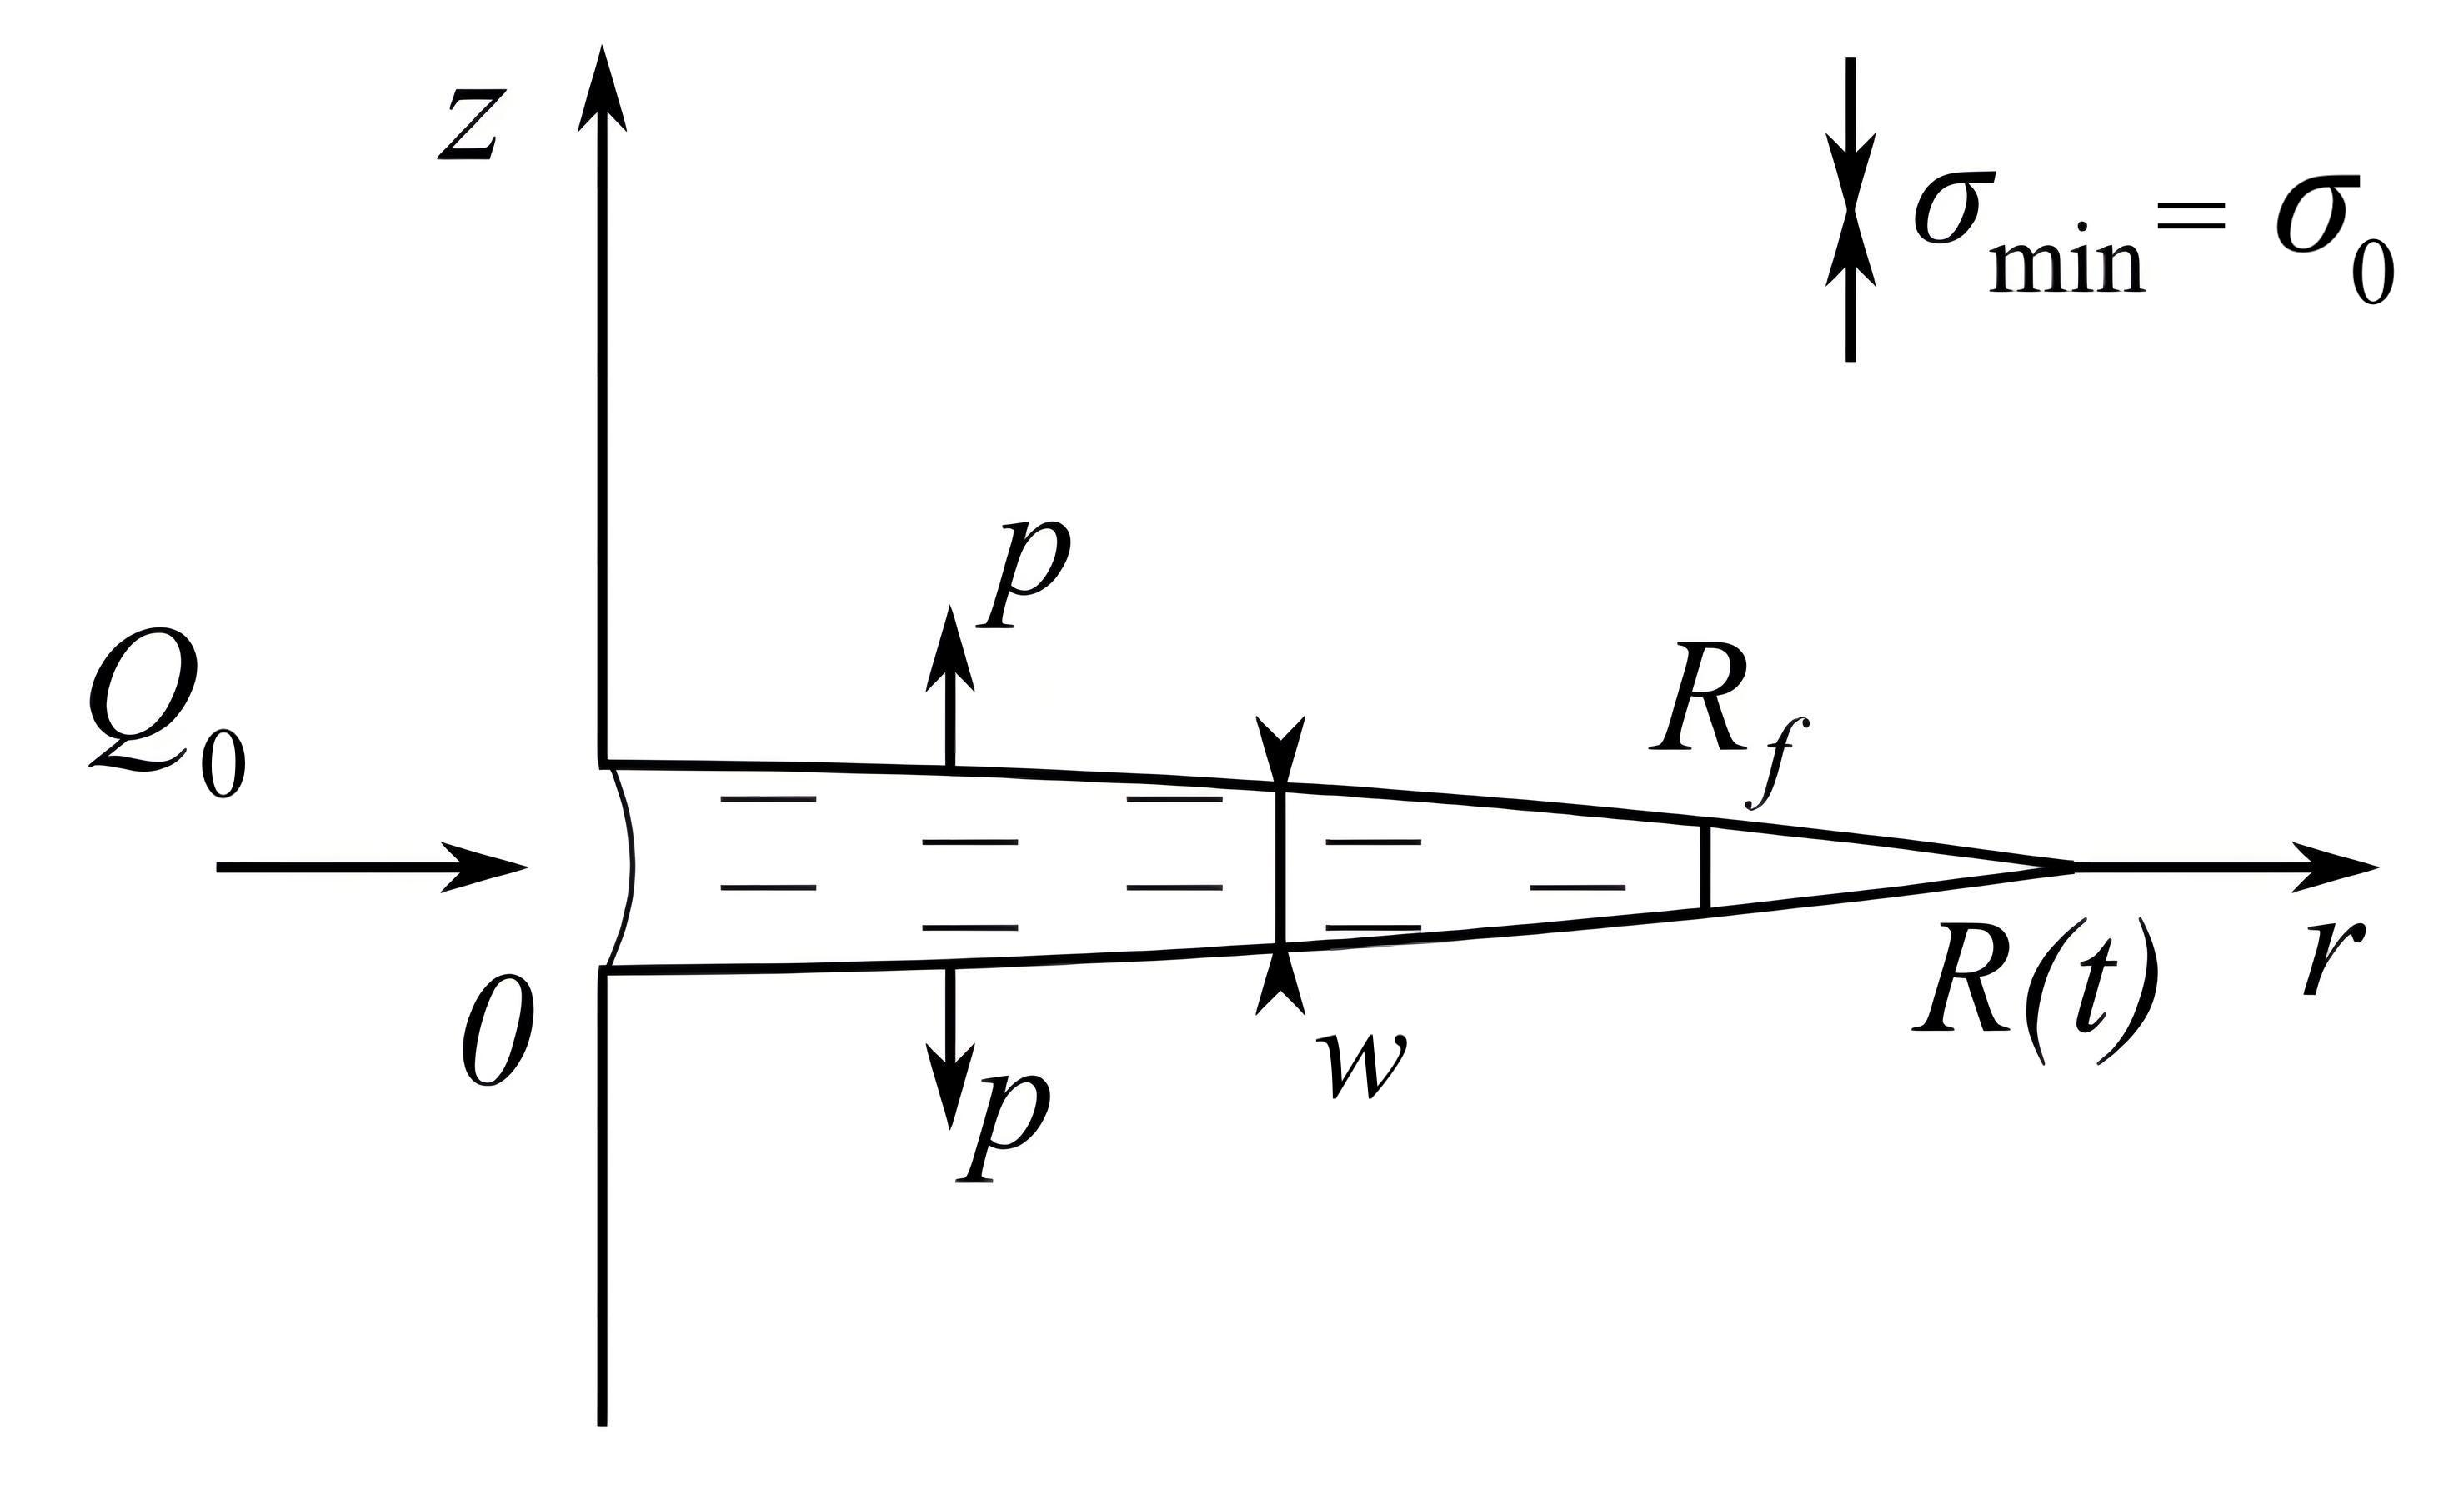
\includegraphics[width=.95\linewidth,valign=t]{images/radial_model_A-A_plane.jpg}
	\end{subfigure}
\captionsetup{justification=centering} %центрировать
\caption{Геометрия радиальной трещины \cite{esipov}: {\itshape a} --- в 3D; {\itshape b} --- проекция A-A} 
\label{fig:radial-model}
\end{figure}


Основные уравнения модели радиальной трещины похожи на уравнения модели KGD.
Основное отличие в том, что теперь рассматривается осесимметричная геометрия в цилиндрической системе координат.
Модель радиальной трещины реализуется в бесконечном по всем направлениям однородном пласте в случае точечного перфорированного интервала.

Радиальные модели трещин применимы при распространении трещин от горизонтальных скважин на ранних временах распространения, так как именно в этом случае длина перфорированного интервала мала и трещина ещё не успела достигнуть границ (кровли и подошвы) пласта.

Система уравнений модели радиальной трещины запишется в цилиндрической системе координат в следующем виде \cite{dontsov2}:

\beq\label{radial_task_111}
\begin{cases}
\dfrac{\partial w}{\partial t}+\dfrac{1}{r}\dfrac{\partial}{\partial r}\left(rq\right)+\dfrac{C'}{\sqrt{t-t_0(r)}}=Q_0\delta(r),\\[15pt]
q=-\dfrac{w^3}{\mu'}\dfrac{\partial p_{\text{net}}}{\partial r},\\[5pt]
p_{\text{net}}(r,t)=-\dfrac{E'}{2\pi R}\displaystyle\int\limits_{0}^{R(t)}\!M\left(\dfrac{r}{R},\dfrac{r'}{R}\right)\dfrac{\partial w(r',t)}{\partial r'}dr',\\[20pt]
\displaystyle\lim_{r\to R}\dfrac{w}{(R-r)^{1/2}}=\dfrac{K'}{E'},
\end{cases}
\eeq
где $C'=2C_l$ -- масштабированный коэффициент одномерных утечек Картера,\newline
\vspace*{3mm}
$\,\,\,\,\,\,\,\;\mu'=12\mu$ -- масштабированная вязкость жидкости,\newline
\vspace*{3mm}
$E'=\dfrac{E}{1-\nu^2}$ -- модуль плоской деформации породы,\newline
\vspace*{4mm}
$\,\,\,K'=\dfrac{8K_{Ic}}{\sqrt{2\pi}}$ -- масштабированная трещиностойкость породы.

Дополнительно в третьем уравнении системы \eqref{radial_task_111} введено чистое (избыточное) давление жидкости в трещине $p_{\text{net}}=p_{\text{frac}}-\sigma_0$, которое представляет собой разность между давлением жидкости в трещине и минимальным горизонтальным напряжением в пласте.\\

Ядро подынтегрального выражения равно
\beq
M\!\left(\rho,s\right)=
\begin{cases}
\dfrac{1}{\rho}K\!\left(\dfrac{s^2}{\rho^2}\right)+\dfrac{\rho}{s^2-\rho^2}E\!\left(\dfrac{s^2}{\rho^2}\right),\,\,\rho>s,\\[15pt]
\dfrac{s}{s^2-\rho^2}E\!\left(\dfrac{\rho^2}{s^2}\right),\,\,\rho<s,
\end{cases}
\eeq
где
$$K(m)=\int\limits_{0}^{\pi/2}{\dfrac{d\varphi}{\sqrt{1-m^2\sin^2{\varphi}}}}$$
и
$$E(m)=\int\limits_{0}^{\pi/2}{\sqrt{1-m^2\sin^2{\varphi}}\,d\varphi}$$
полные эллиптические интегралы первого и второго рода соответственно.
\\

Приближённые решения для модели радиальной трещины во всём параметрическом пространстве представлены в работе \cite{dontsov2}.
Дополнительно в этой же работе \cite{dontsov2} рассмотрены несколько предельных случаев, для которых получены точные аналитические решения, а именно рассмотрены случай доминирования вязкости с доминированием утечек, случай доминирования вязкости с отсутствием утечек, случай доминирования трещиностойкости с доминированием утечек и случай доминирования трещиностойкости с отсутствием утечек.

\section{Модель Перкинса-Керна-Нордгрена (модель PKN)}
\vspace*{-5mm}

\begin{figure}[H]
	\adjustbox{minipage=1.3em,valign=t}{\subcaption{}\label{fig:pkn-model-3D}}%
	\begin{subfigure}[t]{\dimexpr.5\linewidth-1.3em\relax}
		\centering
		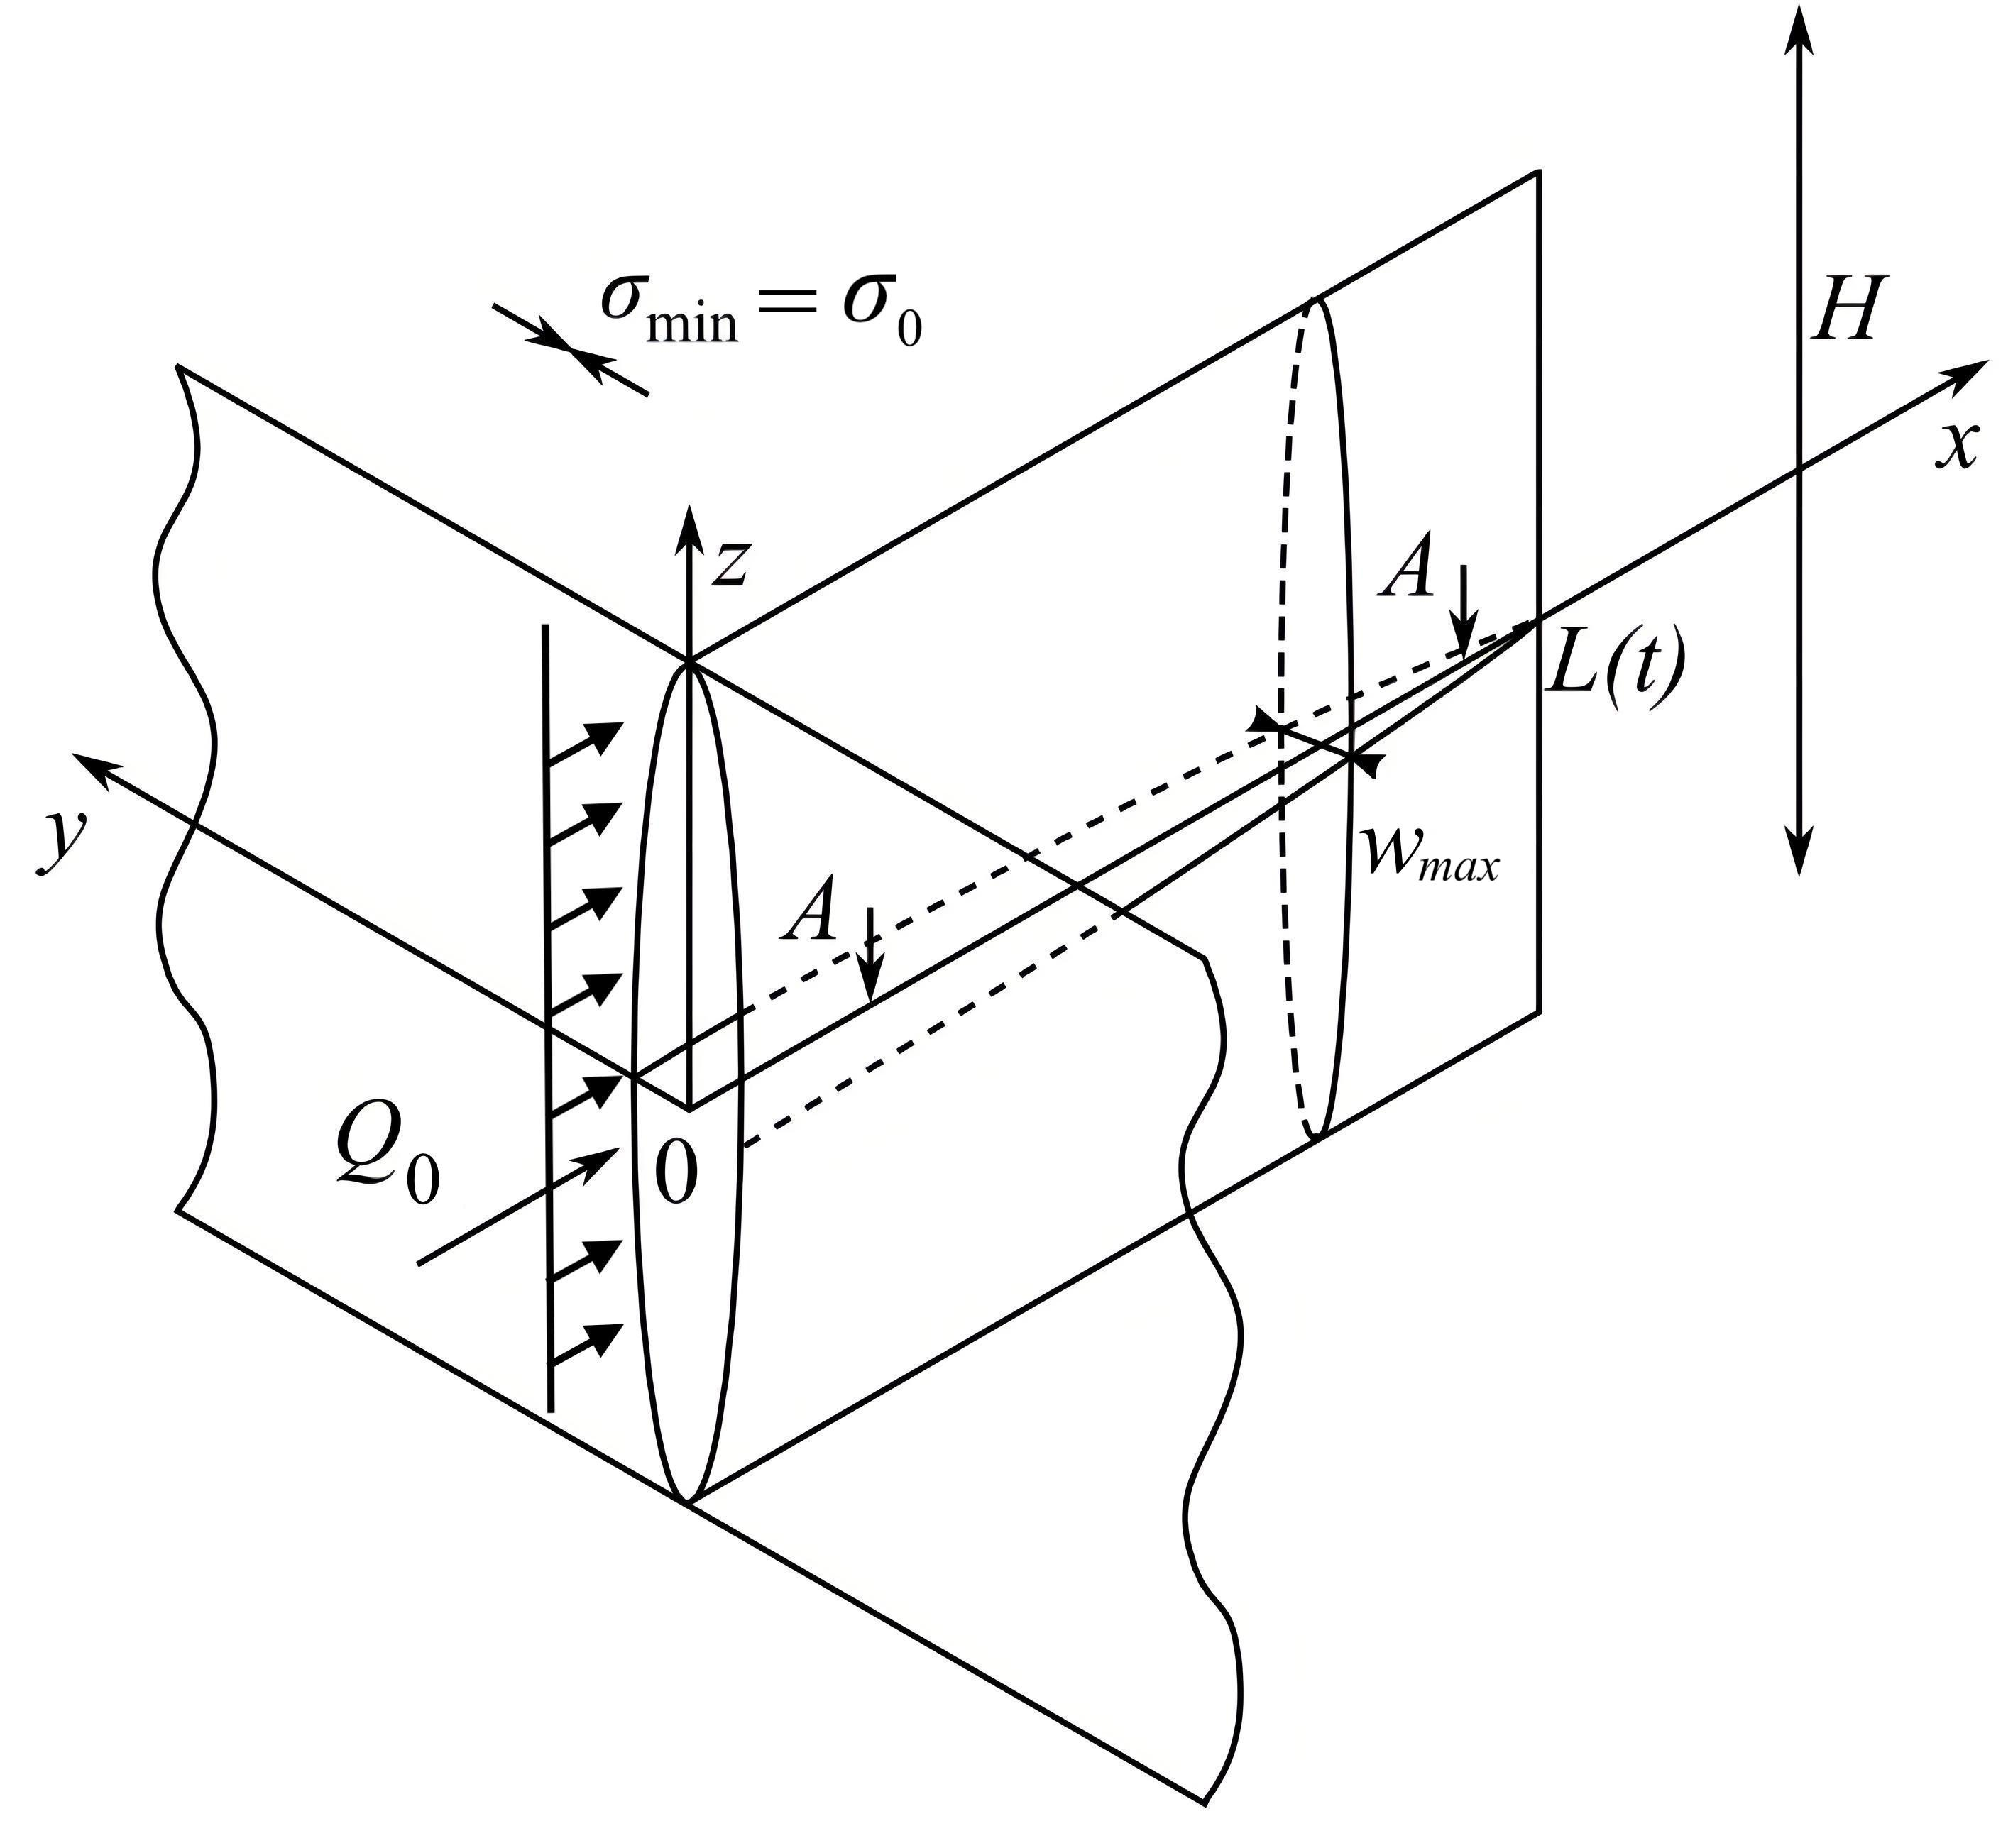
\includegraphics[width=.95\linewidth,valign=t]{images/pkn_model_3D.jpg}
	\end{subfigure}
\hfill %выровнять по ширине
	\adjustbox{minipage=1.3em,valign=t}{\subcaption{}\label{fig:pkn-model-projections}}%
	\begin{subfigure}[t]{\dimexpr.5\linewidth-1.3em\relax}
		\centering
		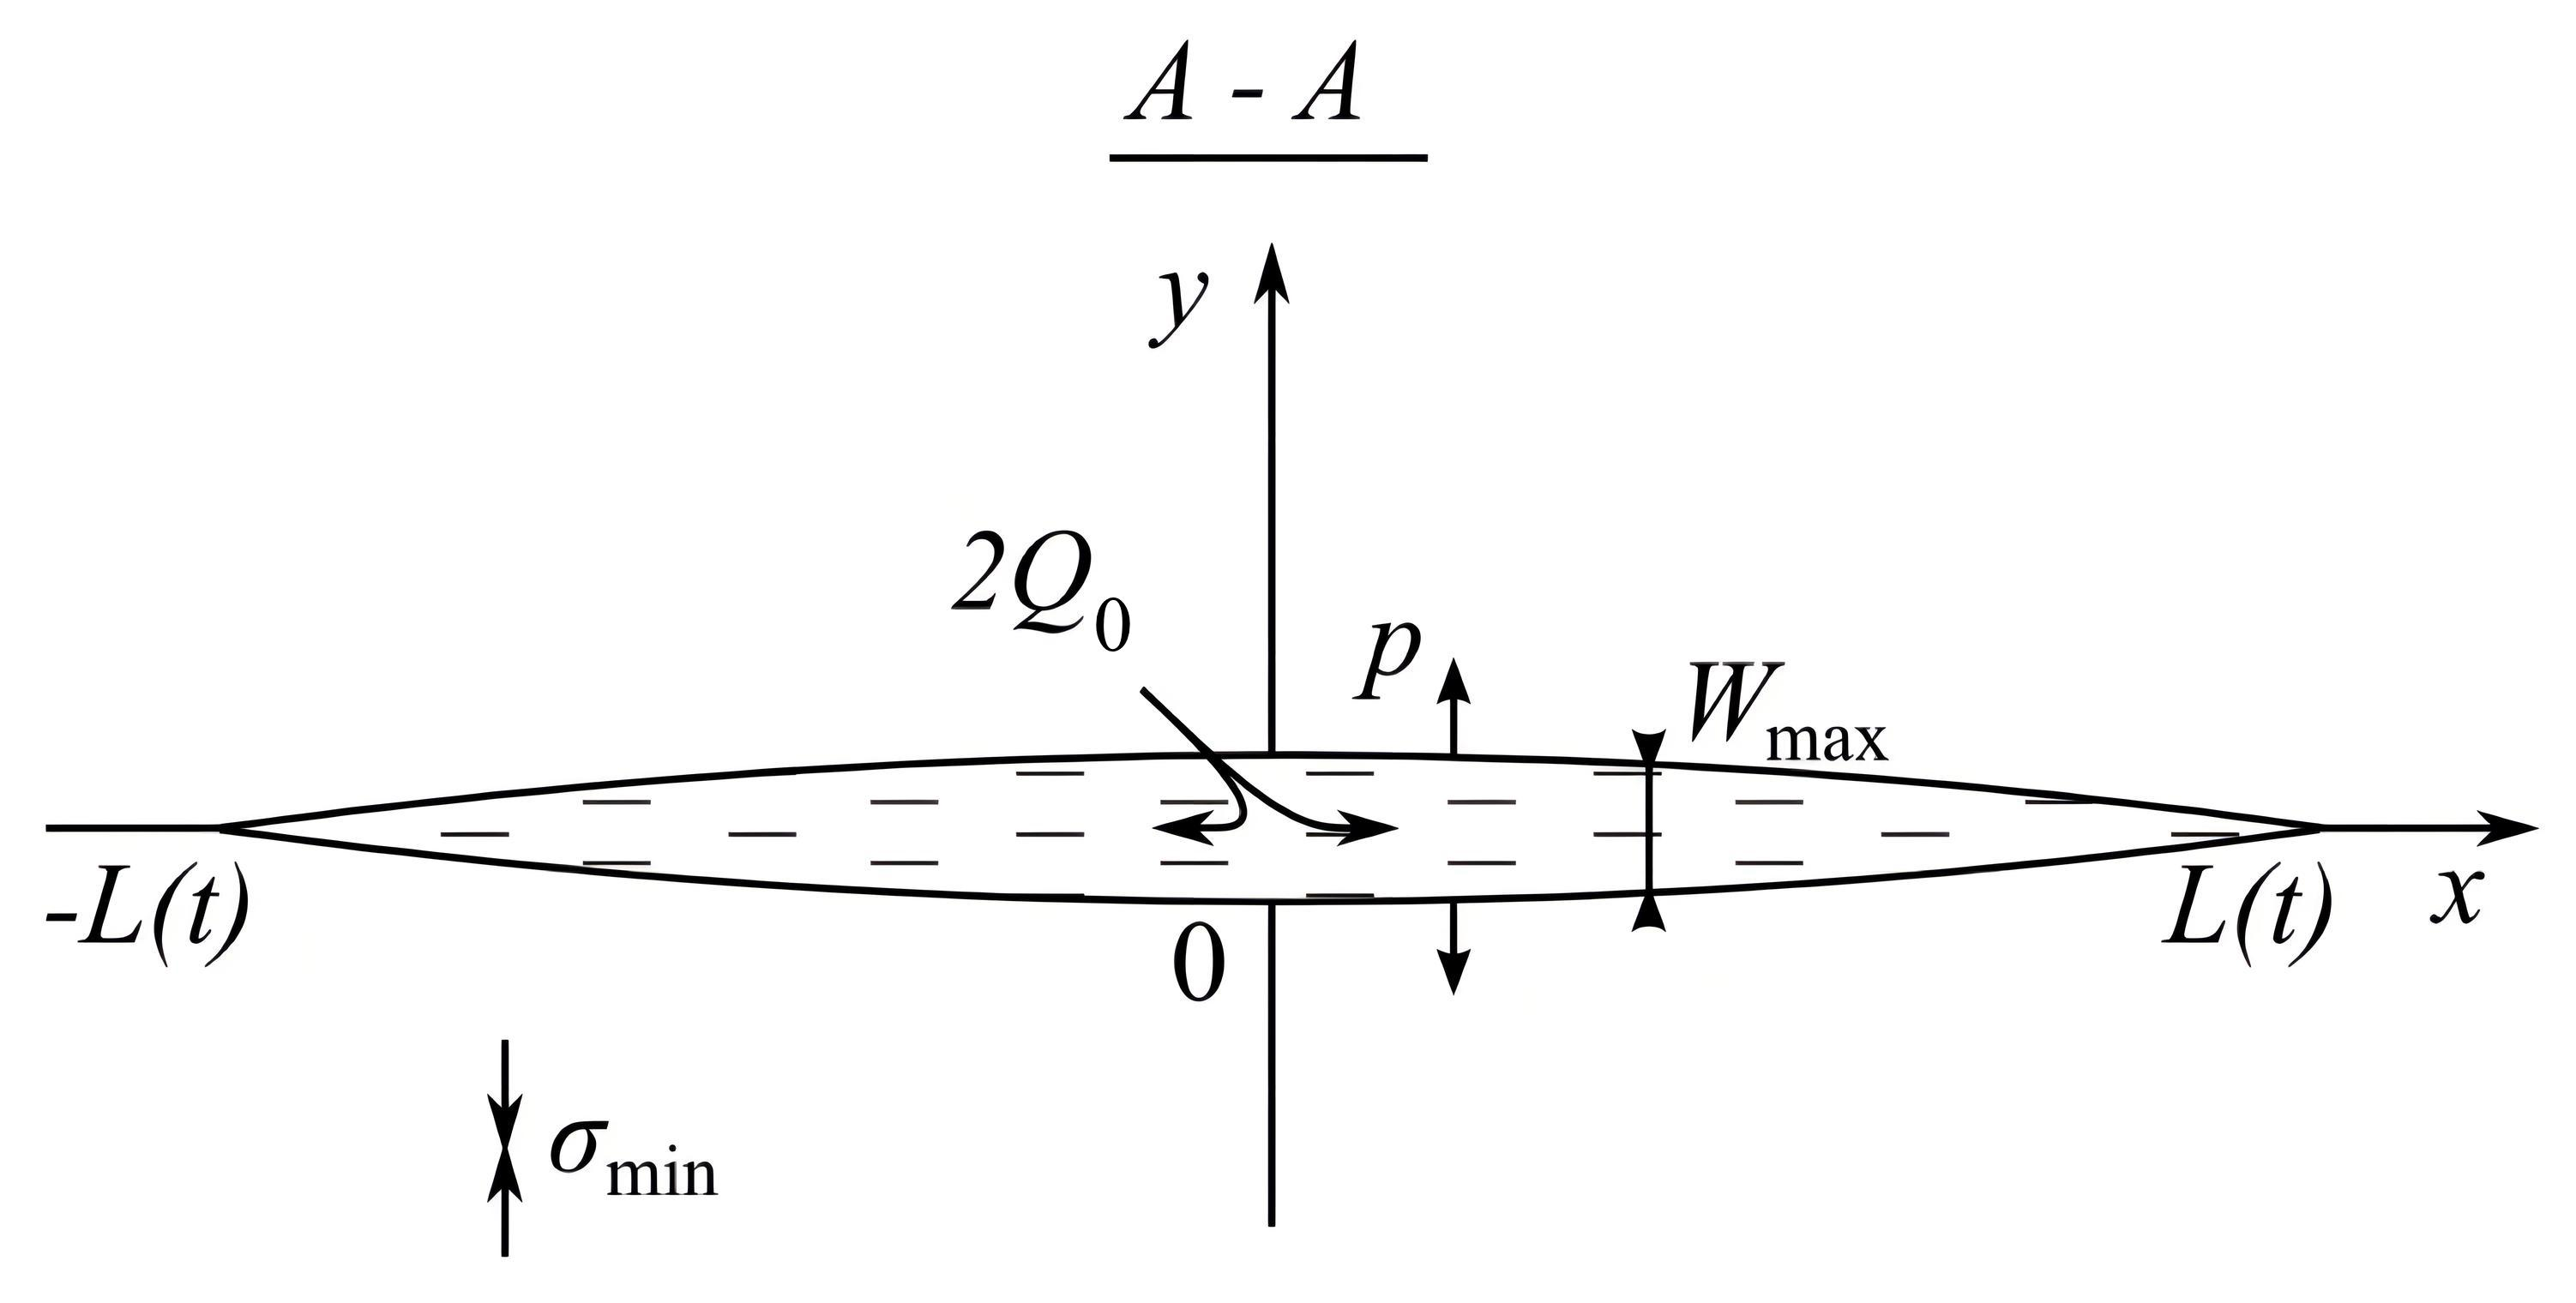
\includegraphics[width=.95\linewidth,valign=t]{images/pkn_model_A-A_plane.jpg}
	\end{subfigure}
\captionsetup{justification=centering} %центрировать
\caption{Геометрия трещины PKN \cite{esipov}: {\itshape a} --- в 3D; {\itshape b} --- проекция A-A} 
\label{fig:pkn-model}
\end{figure}

В модели PKN принимается, что условие плоской деформации сохраняется в каждой вертикальной плоскости, нормальной к направлению распространения; однако, в отличие от ситуации строгой плоской деформации, состояние напряжений и деформаций не точно одинаково в следующих одна за другой плоскостях.
Иными словами, в этой модели используется допущение квази-плоской деформации, причём плоскость отсчёта вертикальна и нормальна к направлению распространения.
В модели PKN пренебрегается изменениями давления вдоль вертикальной координаты, а чистое давление $p_{\text{net}}$ в трещине рассматривается как функция латеральной координаты $x$.

Более строго в модели PKN предполагается, что длина трещины много больше её фиксированной высоты $H$ (отсюда вытекает выполнение условия квази-плоской деформации в вертикальных плоскостях) и в любом вертикальном сечении давление постоянно по сечению.

Из постоянства давления в каждом вертикальном сечении следует эллиптичность вертикального профиля трещины, что позволяет перейти от двумерной системы уравнений к одномерной.
Этот переход осуществляется с помощью аналитического решения вдоль направления оси $Oz$ путём усреднения:
\beq
\bar{w}(x)=\frac{1}{H}\int\limits_{-H/2}^{H/2}{w(x,z)}dz
\eeq
и записи решения вдоль оси $Oz$ в виде эллипса:
\beq
w(x,z)=\frac{4}{\pi}\bar{w}(x)\sqrt{1-\left(\frac{2z}{H}\right)^2}.
\eeq

Система уравнений модели PKN в терминах средних величин (среднее раскрытие и средний поток) запишется в следующем виде:
\beq
\begin{cases}
\dfrac{\partial\bar{w}}{\partial t}+\dfrac{\partial\bar{q}_x}{\partial x}+\dfrac{C'}{\sqrt{t-t_0(x)}}=\dfrac{Q_0}{H}\delta(x),\\[15pt]
\bar{q}_x=-\dfrac{\bar{w}^3}{\pi^2\mu}\dfrac{\partial p_{\text{net}}}{\partial x},\\[15pt]
p_{\text{net}}(x,t)=\dfrac{2E'}{\pi^2H}\displaystyle\int\limits_{-L(t)}^{L(t)}\bar{w}(x',t)\dfrac{dG(2(x'-x)/H)}{dx'}dx',\\[22pt]
\displaystyle\lim_{x\to L}\dfrac{w}{(L-x)^{1/2}}=\dfrac{K'}{E'},
\end{cases}
\eeq
где $C'=2C_l$, $\,\,\,\mu'=12\mu$, $\,\,\,E'=\dfrac{E}{1-\nu^2}$, $\,\,\,K'=\dfrac{8K_{Ic}}{\sqrt{2\pi}}$, $\displaystyle{}\,\,\,G(s)=\frac{\sqrt{1+s^2}}{s}E\left(\frac{1}{1+s^2}\right)$, $\displaystyle{}E(m)=\int\limits_{0}^{\pi/2}{\sqrt{1-m^2\sin^2{\varphi}}\,d\varphi}$.
\\

Приближённые решения для модели трещины PKN во всём параметрическом пространстве и точные аналитические решения для предельных режимов распространения (например, для случая пренебрежимо малой вязкости жидкости и больших утечках) представлены в работе \cite{dontsov2021analysis}.\\

В этой главе были рассмотрены основные модели трещины ГРП.
Для моделирования трещин автоГРП \cite{kalinin} чаще всего используется модель PKN в режиме доминирования трещиностойкости и больших утечках, так как основные предположения модели PKN (длина трещины много больше фиксированной высоты $H$ и давление жидкости в каждом вертикальном сечении постоянно по сечению) соответствуют процессу распространения трещин автоГРП.

В следующей главе будет проведён обзор подходов к моделированию трещин автоГРП.





%\beq
%\frac{\partial\sigma_{xx}}{\partial x}+\frac{\partial\sigma_{xy}}{\partial y}=0
%\eeq


%\section{Название параграфа} \label{ch2:sec1}


